% Options for packages loaded elsewhere
\PassOptionsToPackage{unicode}{hyperref}
\PassOptionsToPackage{hyphens}{url}
\PassOptionsToPackage{dvipsnames,svgnames,x11names}{xcolor}
%
\documentclass[
  letterpaper,
  DIV=11,
  numbers=noendperiod]{scrreprt}

\usepackage{amsmath,amssymb}
\usepackage{iftex}
\ifPDFTeX
  \usepackage[T1]{fontenc}
  \usepackage[utf8]{inputenc}
  \usepackage{textcomp} % provide euro and other symbols
\else % if luatex or xetex
  \usepackage{unicode-math}
  \defaultfontfeatures{Scale=MatchLowercase}
  \defaultfontfeatures[\rmfamily]{Ligatures=TeX,Scale=1}
\fi
\usepackage{lmodern}
\ifPDFTeX\else  
    % xetex/luatex font selection
\fi
% Use upquote if available, for straight quotes in verbatim environments
\IfFileExists{upquote.sty}{\usepackage{upquote}}{}
\IfFileExists{microtype.sty}{% use microtype if available
  \usepackage[]{microtype}
  \UseMicrotypeSet[protrusion]{basicmath} % disable protrusion for tt fonts
}{}
\makeatletter
\@ifundefined{KOMAClassName}{% if non-KOMA class
  \IfFileExists{parskip.sty}{%
    \usepackage{parskip}
  }{% else
    \setlength{\parindent}{0pt}
    \setlength{\parskip}{6pt plus 2pt minus 1pt}}
}{% if KOMA class
  \KOMAoptions{parskip=half}}
\makeatother
\usepackage{xcolor}
\setlength{\emergencystretch}{3em} % prevent overfull lines
\setcounter{secnumdepth}{5}
% Make \paragraph and \subparagraph free-standing
\makeatletter
\ifx\paragraph\undefined\else
  \let\oldparagraph\paragraph
  \renewcommand{\paragraph}{
    \@ifstar
      \xxxParagraphStar
      \xxxParagraphNoStar
  }
  \newcommand{\xxxParagraphStar}[1]{\oldparagraph*{#1}\mbox{}}
  \newcommand{\xxxParagraphNoStar}[1]{\oldparagraph{#1}\mbox{}}
\fi
\ifx\subparagraph\undefined\else
  \let\oldsubparagraph\subparagraph
  \renewcommand{\subparagraph}{
    \@ifstar
      \xxxSubParagraphStar
      \xxxSubParagraphNoStar
  }
  \newcommand{\xxxSubParagraphStar}[1]{\oldsubparagraph*{#1}\mbox{}}
  \newcommand{\xxxSubParagraphNoStar}[1]{\oldsubparagraph{#1}\mbox{}}
\fi
\makeatother


\providecommand{\tightlist}{%
  \setlength{\itemsep}{0pt}\setlength{\parskip}{0pt}}\usepackage{longtable,booktabs,array}
\usepackage{calc} % for calculating minipage widths
% Correct order of tables after \paragraph or \subparagraph
\usepackage{etoolbox}
\makeatletter
\patchcmd\longtable{\par}{\if@noskipsec\mbox{}\fi\par}{}{}
\makeatother
% Allow footnotes in longtable head/foot
\IfFileExists{footnotehyper.sty}{\usepackage{footnotehyper}}{\usepackage{footnote}}
\makesavenoteenv{longtable}
\usepackage{graphicx}
\makeatletter
\def\maxwidth{\ifdim\Gin@nat@width>\linewidth\linewidth\else\Gin@nat@width\fi}
\def\maxheight{\ifdim\Gin@nat@height>\textheight\textheight\else\Gin@nat@height\fi}
\makeatother
% Scale images if necessary, so that they will not overflow the page
% margins by default, and it is still possible to overwrite the defaults
% using explicit options in \includegraphics[width, height, ...]{}
\setkeys{Gin}{width=\maxwidth,height=\maxheight,keepaspectratio}
% Set default figure placement to htbp
\makeatletter
\def\fps@figure{htbp}
\makeatother
% definitions for citeproc citations
\NewDocumentCommand\citeproctext{}{}
\NewDocumentCommand\citeproc{mm}{%
  \begingroup\def\citeproctext{#2}\cite{#1}\endgroup}
\makeatletter
 % allow citations to break across lines
 \let\@cite@ofmt\@firstofone
 % avoid brackets around text for \cite:
 \def\@biblabel#1{}
 \def\@cite#1#2{{#1\if@tempswa , #2\fi}}
\makeatother
\newlength{\cslhangindent}
\setlength{\cslhangindent}{1.5em}
\newlength{\csllabelwidth}
\setlength{\csllabelwidth}{3em}
\newenvironment{CSLReferences}[2] % #1 hanging-indent, #2 entry-spacing
 {\begin{list}{}{%
  \setlength{\itemindent}{0pt}
  \setlength{\leftmargin}{0pt}
  \setlength{\parsep}{0pt}
  % turn on hanging indent if param 1 is 1
  \ifodd #1
   \setlength{\leftmargin}{\cslhangindent}
   \setlength{\itemindent}{-1\cslhangindent}
  \fi
  % set entry spacing
  \setlength{\itemsep}{#2\baselineskip}}}
 {\end{list}}
\usepackage{calc}
\newcommand{\CSLBlock}[1]{\hfill\break\parbox[t]{\linewidth}{\strut\ignorespaces#1\strut}}
\newcommand{\CSLLeftMargin}[1]{\parbox[t]{\csllabelwidth}{\strut#1\strut}}
\newcommand{\CSLRightInline}[1]{\parbox[t]{\linewidth - \csllabelwidth}{\strut#1\strut}}
\newcommand{\CSLIndent}[1]{\hspace{\cslhangindent}#1}

\usepackage{fontspec}
\usepackage{multirow}
\usepackage{multicol}
\usepackage{colortbl}
\usepackage{hhline}
\newlength\Oldarrayrulewidth
\newlength\Oldtabcolsep
\usepackage{longtable}
\usepackage{array}
\usepackage{hyperref}
\usepackage{float}
\usepackage{wrapfig}
\KOMAoption{captions}{tableheading}
\makeatletter
\@ifpackageloaded{bookmark}{}{\usepackage{bookmark}}
\makeatother
\makeatletter
\@ifpackageloaded{caption}{}{\usepackage{caption}}
\AtBeginDocument{%
\ifdefined\contentsname
  \renewcommand*\contentsname{Table of contents}
\else
  \newcommand\contentsname{Table of contents}
\fi
\ifdefined\listfigurename
  \renewcommand*\listfigurename{List of Figures}
\else
  \newcommand\listfigurename{List of Figures}
\fi
\ifdefined\listtablename
  \renewcommand*\listtablename{List of Tables}
\else
  \newcommand\listtablename{List of Tables}
\fi
\ifdefined\figurename
  \renewcommand*\figurename{Figure}
\else
  \newcommand\figurename{Figure}
\fi
\ifdefined\tablename
  \renewcommand*\tablename{Table}
\else
  \newcommand\tablename{Table}
\fi
}
\@ifpackageloaded{float}{}{\usepackage{float}}
\floatstyle{ruled}
\@ifundefined{c@chapter}{\newfloat{codelisting}{h}{lop}}{\newfloat{codelisting}{h}{lop}[chapter]}
\floatname{codelisting}{Listing}
\newcommand*\listoflistings{\listof{codelisting}{List of Listings}}
\makeatother
\makeatletter
\makeatother
\makeatletter
\@ifpackageloaded{caption}{}{\usepackage{caption}}
\@ifpackageloaded{subcaption}{}{\usepackage{subcaption}}
\makeatother

\ifLuaTeX
  \usepackage{selnolig}  % disable illegal ligatures
\fi
\usepackage{bookmark}

\IfFileExists{xurl.sty}{\usepackage{xurl}}{} % add URL line breaks if available
\urlstyle{same} % disable monospaced font for URLs
\hypersetup{
  pdftitle={Title},
  pdfauthor={Canadian Wildlife Federation},
  colorlinks=true,
  linkcolor={blue},
  filecolor={Maroon},
  citecolor={Blue},
  urlcolor={Blue},
  pdfcreator={LaTeX via pandoc}}


\title{Title}
\author{Canadian Wildlife Federation}
\date{29-11-2024}

\begin{document}
\maketitle

\renewcommand*\contentsname{Table of contents}
{
\hypersetup{linkcolor=}
\setcounter{tocdepth}{1}
\tableofcontents
}

\bookmarksetup{startatroot}

\chapter*{Acknowledgements}\label{acknowledgements}
\addcontentsline{toc}{chapter}{Acknowledgements}

\markboth{Acknowledgements}{Acknowledgements}

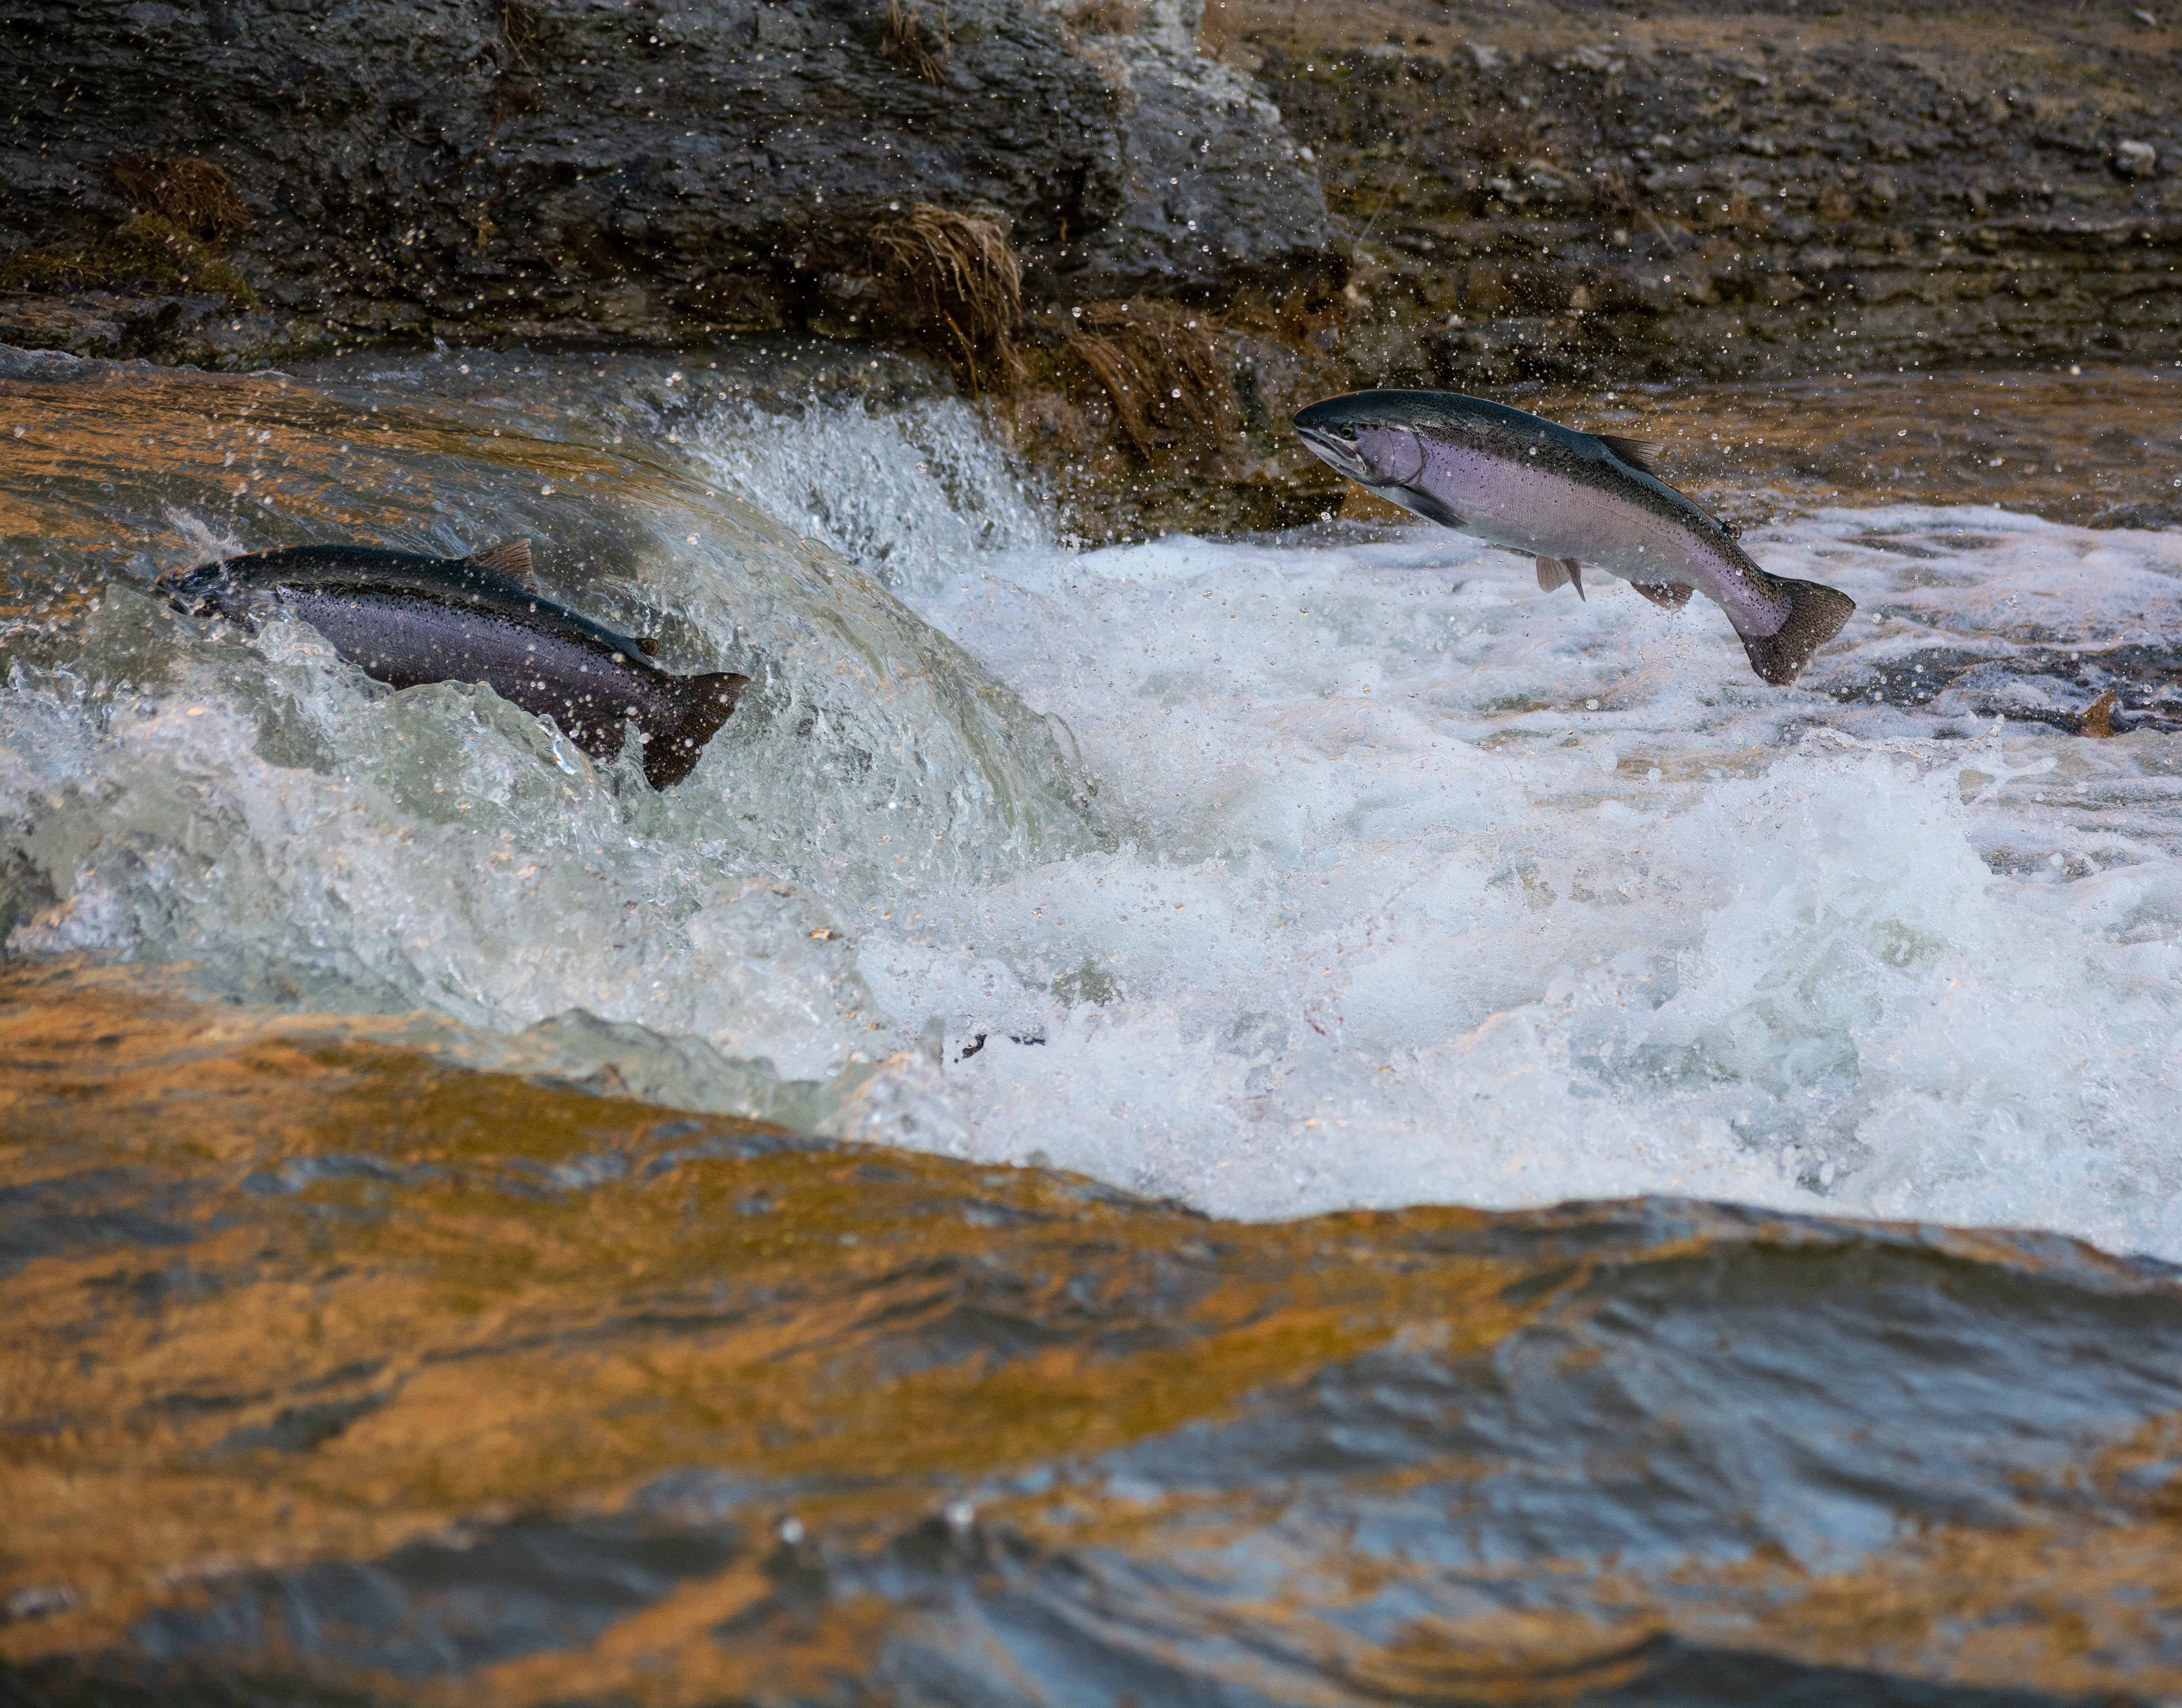
\includegraphics{spawn.jpg}

\bookmarksetup{startatroot}

\chapter*{Project Overview}\label{project-overview}
\addcontentsline{toc}{chapter}{Project Overview}

\markboth{Project Overview}{Project Overview}

\section*{Plan Purpose, Approach, and
Scope}\label{plan-purpose-approach-and-scope}
\addcontentsline{toc}{section}{Plan Purpose, Approach, and Scope}

\markright{Plan Purpose, Approach, and Scope}

The following Watershed Connectivity Restoration Plan (WCRP) represents
the culmination of a collaborative planning effort with the Canadian
Wildlife Federation (CWF), The Atlantic Salmon Federation (ASF), and the
Souris and Area Branch of the PEI Wildlife Federation (SAB). The overall
aim is to build meaningful partnerships, aid in reducing the threat of
aquatic barriers to diadromous fish, and all that they represent, as
well as the livelihoods that they support. This plan will identify
priority actions that the SAB WCRP partners propose to undertake between
2023-2033 to preserve and restore fish connectively in the seven
northeastern salmon watershed systems of North Lake Creek, Priest Pond
Creek, Cross River, Hay River, Bear River, Naufrage River, and Cow River
\{\#fig-geoscope\}. This will be done through barrier rehabilitation and
prevention strategies. These strategies will be shared with local First
Nations, Fisheries and Oceans Canada (DFO), the PEI Government, NGOs,
and local stakeholders to inform directed efforts to improve fish
productivity and diversity in these watersheds.

\section*{Vision Statement}\label{vision-statement}
\addcontentsline{toc}{section}{Vision Statement}

\markright{Vision Statement}

SAB strives to address and remove human and natural barriers in our
managed rivers that could impact movement and the natural life cycles of
aquatic species. SAB will work hard to attain and sustain dynamic
watershed ecosystems with optimal physical, biological, and chemical
conditions to support native wildlife populations and environmental
network functionality so that fish populations can access the habitat
that they need to survive and thrive in throughout their life cycles
without barriers that could distress them. This will allow our local
waterways to be and remain beneficial and healthy for future
generations.

\section*{Project Scope}\label{project-scope}
\addcontentsline{toc}{section}{Project Scope}

\markright{Project Scope}

Connectivity is a critical component of freshwater ecosystems that
encompasses a variety of factors related to ecosystem structure and
function, such as the ability of aquatic organisms to disperse and/or
migrate, the transportation of energy and matter (e.g., nutrient cycling
and sediment flows), and temperature regulation \{cite\}Seliger2018-be.
Though each of these factors are important when considering the health
of a watershed, for the purposes of this WCRP the term ``connectivity''
is defined as the degree to which aquatic organisms can disperse and/or
migrate freely through freshwater systems. Within this context,
connectivity is primarily constrained by physical barriers, including
anthropogenic infrastructure such as dams and stream crossings, and
natural features such as waterfalls, barrier beaches, and beaver dams.
This plan will focus on the direct rehabilitation and prevention of
localized, physical barriers instead of the broad, land-use patterns
causing chronic connectivity issues in the watershed. The planning team
decided that the primary focus of this WCRP is addressing barriers to
longitudinal connectivity (i.e., along the upstream-downstream plane)
due to the importance of maintaining fish passage to spawning and
rearing habitat in the watershed.

\begin{figure}

{\centering \includegraphics{content/images/GeographicScope.png}

}

\caption{Figure 1 - The primary geographic scope, the seven salmon
watersheds --- Bear River, Cow River, Cross River, Hay River, Naufrage
River, North Lake Creek, Priest Pond Creek watershed --- located in
Souris, PE.}

\end{figure}%

The geographic scope of this WCRP is seven watersheds (Bear River, Cow
River, Cross River, Hay River, Naufrage River, North Lake Creek, Priest
Pond Creek) in Souris, PE, (\{numref\}fig1). The seven watersheds have a
total drainage area of 205.46 km2 ranging from 2.5 km2 in Priest Pond to
\textasciitilde49 km2 in North Lake Creek, spanning as far west as
Selkirk and as east as North Lake and draining into the ocean. The
geographic scope of this WCRP was further refined by identifying
naturally accessible waterbodies, which are defined as streams, lakes,
or reservoirs that target species would access in the absence of
anthropogenic barriers (\{numref\}fig2). Naturally accessible
waterbodies were spatially delineated using stream characteristics that
define the upper limit of their movement based on species-specific
swimming abilities (\{numref\}Table1). Areas of high, sustained beaver
activity that has led to long-term changes in the habitat conditions
were excluded due to the unfavorable conditions for barrier remediation.
The spatial extent of the naturally accessible waterbodies layer was
then expanded to include the furthest upstream fish observation data
and/or redd surveys (for Atlantic Salmon). These maps were explored by
the planning team to incorporate additional local knowledge, ensure
accuracy, and finalize the criteria used to define naturally accessible
waterbodies. The new geographic scope formed the foundation for all
subsequent analyses and planning steps, including mapping and modelling
key habitat, quantifying the current connectivity status, goal setting,
and action planning \{cite\}Mazany-Wright2021-rz. The geographic scope
of this WCRP is seven watersheds (Bear River, Cow River, Cross River,
Hay River, Naufrage River, North Lake Creek, Priest Pond Creek) in
Souris, PE, ((\textbf{fig1-geographicscope?})). The seven watersheds
have a total drainage area of 205.46 km2 ranging from 2.5 km2 in Priest
Pond to \textasciitilde49 km2 in North Lake Creek, spanning as far west
as Selkirk and as east as North Lake and draining into the ocean. The
geographic scope of this WCRP was further refined by identifying
naturally accessible waterbodies, which are defined as streams, lakes,
or reservoirs that target species would access in the absence of
anthropogenic barriers (\{numref\}fig2). Naturally accessible
waterbodies were spatially delineated using stream characteristics that
define the upper limit of their movement based on species-specific
swimming abilities (\{numref\}Table1). Areas of high, sustained beaver
activity that has led to long-term changes in the habitat conditions
were excluded due to the unfavorable conditions for barrier remediation.
The spatial extent of the naturally accessible waterbodies layer was
then expanded to include the furthest upstream fish observation data
and/or redd surveys (for Atlantic Salmon). These maps were explored by
the planning team to incorporate additional local knowledge, ensure
accuracy, and finalize the criteria used to define naturally accessible
waterbodies. The new geographic scope formed the foundation for all
subsequent analyses and planning steps, including mapping and modelling
key habitat, quantifying the current connectivity status, goal setting,
and action planning \{cite\}Mazany-Wright2021-rz.

\section*{Focal species}\label{focal-species}
\addcontentsline{toc}{section}{Focal species}

\markright{Focal species}

Focal species represent the ecologically and culturally important
species for which habitat connectivity is being directly conserved
and/or restored in the watershed. The planning team selected three
target species: Atlantic Salmon, Rainbow Smelt, and American Eel. The
selection of these target species was driven primarily by local
conservation goals.

\subsection*{Atlantic Salmon \textbar{} Plamu \textbar{} Salmo
salar}\label{atlantic-salmon-plamu-salmo-salar}
\addcontentsline{toc}{subsection}{Atlantic Salmon \textbar{} Plamu
\textbar{} Salmo salar}

INSERT TEXT here

\subsection*{American Eel \textbar{} Kataq \textbar{} Anguilla
rostrata}\label{american-eel-kataq-anguilla-rostrata}
\addcontentsline{toc}{subsection}{American Eel \textbar{} Kataq
\textbar{} Anguilla rostrata}

::: \{\#tbl-chinook .cell tbl-cap=' table caption'\}

:::

INSERT TEXT

\section*{Structure Types}\label{structure-types}
\addcontentsline{toc}{section}{Structure Types}

\markright{Structure Types}

The following table highlights which structure types pose the greatest
threat to Atlantic Salmon, American Eel, and Rainbow Smelt in the seven
Souris area watersheds. Each structure was assessed for its extent
(i.e., the proportion of the focal species' habitat extent that is
disconnected by all barriers of a given barrier type) and severity
(i.e., the proportion of barrier occurrences that restrict passage to
the focal species). Proportions were either scored as low (1-10\%),
medium (11-30\%), high (31-70\%) or very high (71-100\%)
(\{numref\}Table2). Then, the extent and severity scores were combined
in a matrix to identify an overall threat rating. Ultimately, structure
types that affect a lot of habitat and frequently fully or partially
block fish received the highest ratings. No structures were given a
rating of very high. The results of this assessment exercise were used
to inform the subsequent planning steps, as well as to identify
knowledge gaps where there is little spatial data to inform the
assessment for a specific structure type.

\begin{longtable}[]{@{}lllll@{}}

\caption{\label{tbl-barriertype}SAMPLE Connectivity status assessment
for linear habitat (spawning and rearing).}

\tabularnewline

\caption{}\label{T_2377e}\tabularnewline
\toprule\noalign{}
Barrier Types & Extent & Severity & Irreversibility & Overall Threat
Rating: \\
\midrule\noalign{}
\endfirsthead
\toprule\noalign{}
Barrier Types & Extent & Severity & Irreversibility & Overall Threat
Rating: \\
\midrule\noalign{}
\endhead
\bottomrule\noalign{}
\endlastfoot
Road-Stream Crossings & Low & Low & Medium & Very High \\
Lateral Barriers & High & Very High & High & High \\
Small Dams(\textless3m height) & Low & Low & High & Medium \\
Trail-stream Crossings & Low & Low & Medium & Low \\
Natural Barriers & Medium & High & Low & Low \\

\end{longtable}

\subsection*{Blowdowns/Blockages}\label{blowdownsblockages}
\addcontentsline{toc}{subsection}{Blowdowns/Blockages}

In Sept 2022, Hurricane Fiona caused severe damage to forested areas,
leading to a level of fallen trees that has been estimated to be as
large as 8-10 years' worth of PEI's logging sector harvests (INSERT
CITE). These blowdowns caused physical blockages in the river systems
throughout all seven watersheds and required substantial removal
efforts. Although these areas are not mapped spatially and incorporated
into the estimated connectivity status, clearing blockages was a
significant restoration (management?) effort undertaken by Souris and
Area Branch for the past two years to restore connectivity in these
seven watersheds.

\subsection*{Barrier Beaches}\label{barrier-beaches}
\addcontentsline{toc}{subsection}{Barrier Beaches}

There are five barrier beaches at the mouth of Bear River, Cross River,
Cow River, Hay River, and Priest Pond. These beaches serve as important
estuary habitats where anadromous fish return to, or exit from, during a
portion of their life cycle. The stability of barrier beaches, and
therefore, passability for anadromous species, can depend on factors
such as excessive or diminished sediment supply, rising sea levels
resulting in washouts, and high rates of landward migration and/or
fragmentation (INSERT CITE). Additionally, anthropogenic modifications
of these systems (e.g., rock piles and culverts/fish ladders) enable
further widening and shortening of the estuary, the creation of upstream
reservoirs, and homogenization of stream characteristics, making these
systems more susceptible to instability and blocking fish passage. Cross
River, Cow River, and Priest Pond beaches are considered passable,
whereas Bear River is considered a partial barrier due to its over
widening, shallow channel. At Hay River barrier beach there is a
degraded culvert with a fish ladder on it, and this set of structures
range from partial barrier to salmon and eel to full barrier to Rainbow
Smelt.

\subsection*{Dams}\label{dams}
\addcontentsline{toc}{subsection}{Dams}

There are four mapped dams on naturally accessible waterbodies in the
watersheds, three of which are blocking a total of 24.5 km and 40.8 km
of modelled habitat for American Eel and Atlantic Salmon respectively.
No Rainbow Smelt habitat is located upstream of these dams. Dams impede
passage for all three focal species but have the largest impact on
Rainbow Smelt due to their poor jumping abilities as smaller-bodied
fish. There are two known fish-passage structures associated with dams
in the watersheds; a denil fish ladder on Larkins dam in Naufrage
watershed and a natural bypass channel at Millers dam that leads to a
culvert downstream. Larkins dam was identified on the priority barrier
list (see Appendix B).

\subsection*{Stream Crossings}\label{stream-crossings}
\addcontentsline{toc}{subsection}{Stream Crossings}

Road-stream crossings are the most abundant barrier type in the
watershed, with 181 stream crossings located downstream of modelled key
habitat for either Atlantic Salmon, American Eel, or Rainbow Smelt.
Stream crossings fully or partially block 35.2 km (52\% of habitat
upstream of stream crossings) for Rainbow Smelt, 93.1 (33\%) for salmon
and 103.9 km (61\%). XX\% of assessed crossings have been confirmed as
barriers to fish passage.

\subsection*{Beaver Activity}\label{beaver-activity}
\addcontentsline{toc}{subsection}{Beaver Activity}

INSERT TEXT/LINK to BM plan

\bookmarksetup{startatroot}

\chapter*{Connectivity Status Assessment and
Goals}\label{connectivity-status-assessment-and-goals}
\addcontentsline{toc}{chapter}{Connectivity Status Assessment and Goals}

\markboth{Connectivity Status Assessment and Goals}{Connectivity Status
Assessment and Goals}

\section*{Connectivity Status
Assessment}\label{connectivity-status-assessment}
\addcontentsline{toc}{section}{Connectivity Status Assessment}

\markright{Connectivity Status Assessment}

(see Table~\ref{tbl-connectivity}).

The current connectivity status assessment relies on GIS analyses to map
known and modelled barriers to fish passage, identify stream reaches
that have potential spawning and rearing habitat, estimate the
proportion of habitat that is currently accessible to target species,
and prioritize barriers for field assessment that would provide the
greatest gains in connectivity. To support a flexible prioritization
framework to identify priority barriers in the watershed, two
assumptions are made: 1,any modelled (i.e., passability status is
unknown) or partial barriers are treated as complete barriers to passage
and 2, the habitat modelling is binary, it does not assign any habitat
quality values. As such, the current connectivity status will be refined
over time as more data on habitat and barriers are collected. For more
detail on how the connectivity status assessments were conducted, see
Data Download and Methods.

\begin{longtable}[]{@{}lllllll@{}}

\caption{\label{tbl-connectivity}SAMPLE TABLE Connectivity status
assessment for spawning and rearing habitat.}

\tabularnewline

\caption{}\label{T_cf2e2}\tabularnewline
\toprule\noalign{}
Target Species & KEA & Indicator & Poor & Fair & Good & Very Good \\
\midrule\noalign{}
\endfirsthead
\toprule\noalign{}
Target Species & KEA & Indicator & Poor & Fair & Good & Very Good \\
\midrule\noalign{}
\endhead
\bottomrule\noalign{}
\endlastfoot
Andromous Salmon & Available Spawning Habitat & \% of total habitat &
\textless50\% & 51-75\% & 76-90\% & \textgreater90\% \\
& & Current Status: & & & & 92 \\

\end{longtable}

\section*{Goals}\label{goals}
\addcontentsline{toc}{section}{Goals}

\markright{Goals}

\begin{longtable}[]{@{}ll@{}}

\caption{\label{tbl-goals}SAMPLE TABLE Goals to improve spawning and
rearing habitat connectivity for target species in the watershed. The
goals were established through discussions with the planning team and
represent the resulting desired state of connectivity in the watershed.
The goals are subject to change as more information and data are
collected over the course of the plan timeline (e.g., the current
connectivity status is updated based on barrier field assessments).}

\tabularnewline

\caption{}\label{T_02248}\tabularnewline
\toprule\noalign{}
Goal \# & Goal \\
\midrule\noalign{}
\endfirsthead
\toprule\noalign{}
Goal \# & Goal \\
\midrule\noalign{}
\endhead
\bottomrule\noalign{}
\endlastfoot
1 & By 2040, the percent (\%) of total linear habitat accessible to
anadromous salmon will increase from 92\% to 96\% within the Horsefly
River watershed (i.e., reconnect at least 14.77 km of habitat). \\
2 & By 2024, the total area of overwintering habitat accessible to
Anadromous Salmon will increase by 1,500 m2 within the Horsefly River
watershed. \\

\end{longtable}

\bookmarksetup{startatroot}

\chapter*{Barrier Prioritization}\label{barrier-prioritization}
\addcontentsline{toc}{chapter}{Barrier Prioritization}

\markboth{Barrier Prioritization}{Barrier Prioritization}

\section*{\texorpdfstring{ Barrier Prioritization
Summary}{ Barrier Prioritization Summary}}\label{barrier-prioritization-summary}
\addcontentsline{toc}{section}{ Barrier Prioritization Summary}

\markright{ Barrier Prioritization Summary}

The primary conservation outcome of the WCRP will be \ldots{} To achieve
this, it is necessary to prioritize and identify a suite of barriers
that, if remediated, will provide access to a minimum of 14.77 km of
spawning or rearing habitat (Table~\ref{tbl-gainReqs}):

\begin{longtable}[]{@{}llllll@{}}

\caption{\label{tbl-gainReqs}SAMPLE Spawning and rearing habitat
connectivity gain requirements to meet WCRP goals in . The measures of
currently accessible and total habitat values are derived from the
Intrinsic Potential habitat model.}

\tabularnewline

\caption{}\label{T_ab7f3}\tabularnewline
\toprule\noalign{}
Habitat Type & Currently accessible (km) & Total & Current Connectivity
Status & Goal & Gain required (km) \\
\midrule\noalign{}
\endfirsthead
\toprule\noalign{}
Habitat Type & Currently accessible (km) & Total & Current Connectivity
Status & Goal & Gain required (km) \\
\midrule\noalign{}
\endhead
\bottomrule\noalign{}
\endlastfoot
Spawning and Rearing & 326.28 & 355.26 & 92\% & 96\% & 14.77 \\

\end{longtable}

The barrier prioritization analysis ranked barriers by {[}\ldots{]} A
longer list of barriers is needed due to the inherent assumptions in the
connectivity model, habitat model, and gaps in available data. Barriers
that have been modelled (i.e., points where streams and road/rail
networks intersect) are assumed to be barriers until field verification
is undertaken and structures that have been assessed as ``potential''
barriers (e.g., may be passable at certain flow levels or for certain
life history stages) require further investigation before a definitive
remediation decision is made. Additionally, the habitat model identifies
stream segments that have the potential to support spawning or rearing
habitat for target species but does not attempt to quantify habitat
quality or suitability (see Appendix B), which will require additional
field verification once barrier assessments have completed.Data
deficient structures represents structures that are a priority to
evaluate further through barrier assessment and habitat confirmations
because some structures will likely be passable, others will not be
associated with usable habitat, and others may not be feasible to
remediate because of logistic considerations
(Table~\ref{tbl-deficient}). Some barriers were moved forward to the
``priority barrier list'' (see Table~\ref{tbl-priority}) and others were
eliminated from consideration due to one or more of the considerations
discussed above (see Table~\ref{tbl-remove}). The priority barrier list
represents structures that were confirmed to be partial or full barriers
to fish passage and that block access to confirmed habitat. Barriers on
the priority list were reviewed by planning team members and selected
for inclusion for proactive pursual of remediation. For more details on
the barrier prioritization model, please see Mazany-Wright et al.
(2021).

\begin{table}

\caption{\label{tbl-priority}SAMPLE priority barrier list, which
includes barriers that have undergone field assessment, been reviewed by
the planning team, and selected to pursue for proactive remediation.}

\centering{

The dataset is empty. No table to display.

}

\end{table}%

\begin{table}

\caption{\label{tbl-deficient}Assessed structures that remain data
deficient}

\centering{

The dataset is empty. No table to display.

}

\end{table}%

\begin{table}

\caption{\label{tbl-remove}List of barriers that were prioritized as
part of the first iteration but were removed from consideration for
pursual of proactive remediation following discussion with the planning
team due to these structures not existing, being passable, not be
associated with usable habitat, or deemed not feasible to remediate
because of logistic considerations.}

\centering{

The dataset is empty. No table to display.

}

\end{table}%

Out of the 0 on the intermediate list, 16 require further field
assessment before selection as a final barrier to pursue for
remediation:

There are currently 0 barriers on the priority barrier list, which will
be pursued for proactive remediation to achieve the connectivity goals
in this plan:

\begin{table}

\caption{\label{tbl-rehab}Rehabilitated structures.}

\centering{

The dataset is empty. No table to display.

}

\end{table}%

\bookmarksetup{startatroot}

\chapter*{Work Planning}\label{work-planning}
\addcontentsline{toc}{chapter}{Work Planning}

\markboth{Work Planning}{Work Planning}

\section*{Annual Progress Report}\label{annual-progress-report}
\addcontentsline{toc}{section}{Annual Progress Report}

\markright{Annual Progress Report}

\section*{Operational Plan}\label{operational-plan}
\addcontentsline{toc}{section}{Operational Plan}

\markright{Operational Plan}

The operational plan represents a preliminary exercise undertaken by the
planning team to identify the potential leads, potential participants,
and estimated cost for the implementation of each action in . The table
below summarizes individuals, groups, or organizations that the planning
team felt could lead or participate in the implementation of the plan
and should be interpreted as the first step in on-going planning and
engagement to develop more detailed and sophisticated action plans for
each entry in the table. The individuals, groups, and organizations
listed under the ``Lead(s)'' or ``Potential Participants'' columns are
those that provisionally expressed interest in participating in one of
those roles or were suggested by the planning team for further
engagement (denoted in bold), for those that are not members of the
planning team. The leads, participants, and estimated costs in the
operational plan are not binding nor an official commitment of
resources, but rather provide a roadmap for future coordination and
engagement to work towards implementation of the WCRP.

\begin{longtable}[]{@{}llll@{}}

\caption{\label{tbl-opplan}Operational plan to support the
implementation of strategies and actions to improve connectivity for
target species in .}

\tabularnewline

\caption{}\label{T_89864}\tabularnewline
\toprule\noalign{}
Strategy / Actions & Lead(s) {[}1{]} & Participants3 & Total Budget \\
\midrule\noalign{}
\endfirsthead
\toprule\noalign{}
Strategy / Actions & Lead(s) {[}1{]} & Participants3 & Total Budget \\
\midrule\noalign{}
\endhead
\bottomrule\noalign{}
\endlastfoot
Strategy 1: Crossing Remediation & & & \$3,666,300.00 \\
1.1 -- Remediate crossings that are acting as barriers & CWF & Horsefly
River Roundtable, Fisheries and Oceans Canada (DFO) & \$3,500,000.00 \\
1.2 -- Lobby that the government enforce their regulations & TBD & CWF,
Horsefly River Roundtable, Williams Lake First Nation (WLFN) &
\$10,000.00 \\
1.3 -- Initiate a barrier owner outreach program for locations on the
barrier remediation shortlist & HRR, CWF, DFO & & TBD \\
1.4 -- Knowledge Gap: Continue updating the barrier prioritization model
& CWF & TBD & \$100,000.00 \\
1.5 -- Knowledge Gap: conduct field assessments on updated preliminary
barrier list using the provincial fish passage framework and update
connectivity goal if additional barriers are added to the barrier
remediation shortlist & CWF & Horsefly River Roundtable, DFO &
\$50,300.00 \\
1.6 - Update longitudinal connectivity goal if additional barriers are
added to the barrier remediation shortlist & & & \\
1.7 -- Knowledge Gap: Identify and map crossing ownership for barriers
on the barrier remediation shortlist & TBD & CWF, DFO (Anthonie) &
\$1,500.00 \\
1.8 -- Knowledge Gap: Compile road maintenance schedules & DFO & CWF,
WLFN, DFO, FLNRORD & \$2,000.00 \\
1.9 -- Knowledge Gap: Survey trail-stream crossings to confirm low
pressure rating values & WLFN & CWF, DFO & \$2,500.00 \\
Strategy 2: Lateral Barrier Remediation & & & \$80,000.00 \\
2.1 -- Remediate dikes / berms / other structures that are acting as
barriers & CWF & DFO, Horsefly River Roundtable & TBD \\
2.2 -- Initiate a barrier owner outreach program & TBD & CWF, DFO &
TBD \\
2.3 -- Knowledge Gap: Identify and map year-round lateral habitat, as
well as overwintering habitat & Horsefly River Roundtable, DFO & CWF,
Northern Shuswap Tribal Council (NSTC), WLFN & \$65,000.00 \\
2.4 -- Knowledge Gap: Map lateral barriers and barrier ownership & CWF &
DFO, Horsefly River Roundtable & \$5,000.00 \\
2.5 -- Knowledge Gap: Develop a framework to assess and prioritize
between different lateral barrier remediation projects & CWF & DFO &
\$10,000.00 \\
Strategy 3: Dam Remediation & & & \$1,305,000.00 \\
3.1 - Remediate Dams & TBD & TBD & \$1,305,000.00 \\
3.2 - Install Fish Passage & TBD & TBD & TBD \\
3.3 - Connect with Cattleman\textquotesingle s Association to explore a
partnership to remediate dams & TBD & TBD & TBD \\
3.4 - Knowledge Gap: Continue updating the barrier prioritization model
& CWF & TBD & \$0.00 \\
3.5 - Knowledge Gap: Assess dams to determine whether they exist and are
truly blocking salmon habitat & HRR(?) DFO(?) CWF(?) & TBD & TBD \\
3.6 - Knowledge Gap: Identify and map dam ownership & TBD & TBD & TBD \\
Strategy 4: Barrier Prevention & & & \$110,000.00 \\
4.1 -- Explore potential partnerships with industrial companies & TBD &
CWF, DFO, Horsefly River Roundtable, WLFN & \$10,000.00 \\
4.2 -- Stabilize sediment sources that are explicitly linked to sediment
wedges or erosion that are acting as barriers & TBD & DFO &
\$100,000.00 \\
Strategy 5: Progress Tracking Plan & & & TBD \\
5.1 - Implement the WCRP Progress Tracking Plan & CWF & & TBD \\
5.2 - Develop a communication action to raise awareness and support for
this WCRP & CWF, HRR & TBD & TBD \\
Total: & & & \$5,161,300.00 \\
Fundraising total: & & & \$2,508,800 \\
Proponent/government contribution total: & & & \$2,652,500 \\

\end{longtable}

\section*{Annual Work Plan}\label{annual-work-plan}
\addcontentsline{toc}{section}{Annual Work Plan}

\markright{Annual Work Plan}

\bookmarksetup{startatroot}

\chapter*{References}\label{references}
\addcontentsline{toc}{chapter}{References}

\markboth{References}{References}

\phantomsection\label{refs}
\begin{CSLReferences}{1}{0}
\bibitem[\citeproctext]{ref-Mazany-Wright2021-rz}
Mazany-Wright, N, S M Norris, N W R Lapointe, and B Rebellato. 2021.
{``A Freshwater Connectivity Modelling Framework to Support Barrier
Prioritization and Remediation in British Columbia.''} \emph{Canadian
Wildlife Federation}.

\end{CSLReferences}

\bookmarksetup{startatroot}

\chapter*{Version History}\label{version-history}
\addcontentsline{toc}{chapter}{Version History}

\markboth{Version History}{Version History}

\cleardoublepage
\phantomsection
\addcontentsline{toc}{part}{Appendices}
\appendix

\chapter*{Project Partners}\label{project-partners}
\addcontentsline{toc}{chapter}{Project Partners}

\markboth{Project Partners}{Project Partners}

\section*{Planning Team}\label{planning-team}
\addcontentsline{toc}{section}{Planning Team}

\markright{Planning Team}

\global\setlength{\Oldarrayrulewidth}{\arrayrulewidth}

\global\setlength{\Oldtabcolsep}{\tabcolsep}

\setlength{\tabcolsep}{2pt}

\renewcommand*{\arraystretch}{1.5}



\providecommand{\ascline}[3]{\noalign{\global\arrayrulewidth #1}\arrayrulecolor[HTML]{#2}\cline{#3}}

\begin{longtable}[c]{|p{1.65in}|p{4.35in}}

\caption{\label{tbl-planteam}SAMPLE WCRP planning team members. Planning
team members contributed to the development of this plan by
participating in a series of workshops and document and data review. The
plan was generated based on the input and feedback of the local groups
and organizations listed in this table.}

\tabularnewline

\hhline{>{\arrayrulecolor[HTML]{666666}\global\arrayrulewidth=1.5pt}->{\arrayrulecolor[HTML]{666666}\global\arrayrulewidth=1.5pt}-}

\multicolumn{1}{>{\cellcolor[HTML]{008270}\raggedright}m{\dimexpr 1.65in+0\tabcolsep}}{\textcolor[HTML]{FFFFFF}{\fontsize{11}{11}\selectfont{\global\setmainfont{Arial}{Name}}}} & \multicolumn{1}{>{\cellcolor[HTML]{008270}\raggedright}m{\dimexpr 4.35in+0\tabcolsep}}{\textcolor[HTML]{FFFFFF}{\fontsize{11}{11}\selectfont{\global\setmainfont{Arial}{Organization}}}} \\

\noalign{\global\arrayrulewidth 0pt}\arrayrulecolor[HTML]{000000}

\hhline{>{\arrayrulecolor[HTML]{666666}\global\arrayrulewidth=1.5pt}->{\arrayrulecolor[HTML]{666666}\global\arrayrulewidth=1.5pt}-}\endfirsthead 

\hhline{>{\arrayrulecolor[HTML]{666666}\global\arrayrulewidth=1.5pt}->{\arrayrulecolor[HTML]{666666}\global\arrayrulewidth=1.5pt}-}

\multicolumn{1}{>{\cellcolor[HTML]{008270}\raggedright}m{\dimexpr 1.65in+0\tabcolsep}}{\textcolor[HTML]{FFFFFF}{\fontsize{11}{11}\selectfont{\global\setmainfont{Arial}{Name}}}} & \multicolumn{1}{>{\cellcolor[HTML]{008270}\raggedright}m{\dimexpr 4.35in+0\tabcolsep}}{\textcolor[HTML]{FFFFFF}{\fontsize{11}{11}\selectfont{\global\setmainfont{Arial}{Organization}}}} \\

\noalign{\global\arrayrulewidth 0pt}\arrayrulecolor[HTML]{000000}

\hhline{>{\arrayrulecolor[HTML]{666666}\global\arrayrulewidth=1.5pt}->{\arrayrulecolor[HTML]{666666}\global\arrayrulewidth=1.5pt}-}\endhead



\multicolumn{1}{>{\raggedright}m{\dimexpr 1.65in+0\tabcolsep}}{\textcolor[HTML]{000000}{\fontsize{11}{11}\selectfont{\global\setmainfont{Arial}{Betty\ Rebellato}}}} & \multicolumn{1}{>{\raggedright}m{\dimexpr 4.35in+0\tabcolsep}}{\textcolor[HTML]{000000}{\fontsize{11}{11}\selectfont{\global\setmainfont{Arial}{Canadian\ Wildlife\ Federation}}}} \\

\noalign{\global\arrayrulewidth 0pt}\arrayrulecolor[HTML]{000000}





\multicolumn{1}{>{\raggedright}m{\dimexpr 1.65in+0\tabcolsep}}{\textcolor[HTML]{000000}{\fontsize{11}{11}\selectfont{\global\setmainfont{Arial}{Nick\ Mazany-Wright}}}} & \multicolumn{1}{>{\raggedright}m{\dimexpr 4.35in+0\tabcolsep}}{\textcolor[HTML]{000000}{\fontsize{11}{11}\selectfont{\global\setmainfont{Arial}{Canadian\ Wildlife\ Federation}}}} \\

\noalign{\global\arrayrulewidth 0pt}\arrayrulecolor[HTML]{000000}





\multicolumn{1}{>{\raggedright}m{\dimexpr 1.65in+0\tabcolsep}}{\textcolor[HTML]{000000}{\fontsize{11}{11}\selectfont{\global\setmainfont{Arial}{Nicolas\ Lapointe}}}} & \multicolumn{1}{>{\raggedright}m{\dimexpr 4.35in+0\tabcolsep}}{\textcolor[HTML]{000000}{\fontsize{11}{11}\selectfont{\global\setmainfont{Arial}{Canadian\ Wildlife\ Federation}}}} \\

\noalign{\global\arrayrulewidth 0pt}\arrayrulecolor[HTML]{000000}





\multicolumn{1}{>{\raggedright}m{\dimexpr 1.65in+0\tabcolsep}}{\textcolor[HTML]{000000}{\fontsize{11}{11}\selectfont{\global\setmainfont{Arial}{Sarah\ Sra}}}} & \multicolumn{1}{>{\raggedright}m{\dimexpr 4.35in+0\tabcolsep}}{\textcolor[HTML]{000000}{\fontsize{11}{11}\selectfont{\global\setmainfont{Arial}{Canadian\ Wildlife\ Federation}}}} \\

\noalign{\global\arrayrulewidth 0pt}\arrayrulecolor[HTML]{000000}





\multicolumn{1}{>{\raggedright}m{\dimexpr 1.65in+0\tabcolsep}}{\textcolor[HTML]{000000}{\fontsize{11}{11}\selectfont{\global\setmainfont{Arial}{Colin\ McGregor}}}} & \multicolumn{1}{>{\raggedright}m{\dimexpr 4.35in+0\tabcolsep}}{\textcolor[HTML]{000000}{\fontsize{11}{11}\selectfont{\global\setmainfont{Arial}{Department\ of\ Fisheries\ and\ Oceans\ Canada}}}} \\

\noalign{\global\arrayrulewidth 0pt}\arrayrulecolor[HTML]{000000}





\multicolumn{1}{>{\raggedright}m{\dimexpr 1.65in+0\tabcolsep}}{\textcolor[HTML]{000000}{\fontsize{11}{11}\selectfont{\global\setmainfont{Arial}{Guy\ Scharf}}}} & \multicolumn{1}{>{\raggedright}m{\dimexpr 4.35in+0\tabcolsep}}{\textcolor[HTML]{000000}{\fontsize{11}{11}\selectfont{\global\setmainfont{Arial}{Department\ of\ Fisheries\ and\ Oceans\ Canada}}}} \\

\noalign{\global\arrayrulewidth 0pt}\arrayrulecolor[HTML]{000000}





\multicolumn{1}{>{\raggedright}m{\dimexpr 1.65in+0\tabcolsep}}{\textcolor[HTML]{000000}{\fontsize{11}{11}\selectfont{\global\setmainfont{Arial}{Thomas\ Gristey}}}} & \multicolumn{1}{>{\raggedright}m{\dimexpr 4.35in+0\tabcolsep}}{\textcolor[HTML]{000000}{\fontsize{11}{11}\selectfont{\global\setmainfont{Arial}{Department\ of\ Fisheries\ and\ Oceans\ Canada}}}} \\

\noalign{\global\arrayrulewidth 0pt}\arrayrulecolor[HTML]{000000}





\multicolumn{1}{>{\raggedright}m{\dimexpr 1.65in+0\tabcolsep}}{\textcolor[HTML]{000000}{\fontsize{11}{11}\selectfont{\global\setmainfont{Arial}{Simon\ Norris}}}} & \multicolumn{1}{>{\raggedright}m{\dimexpr 4.35in+0\tabcolsep}}{\textcolor[HTML]{000000}{\fontsize{11}{11}\selectfont{\global\setmainfont{Arial}{Hillcrest\ Geographics}}}} \\

\noalign{\global\arrayrulewidth 0pt}\arrayrulecolor[HTML]{000000}





\multicolumn{1}{>{\raggedright}m{\dimexpr 1.65in+0\tabcolsep}}{\textcolor[HTML]{000000}{\fontsize{11}{11}\selectfont{\global\setmainfont{Arial}{Brian\ Englund}}}} & \multicolumn{1}{>{\raggedright}m{\dimexpr 4.35in+0\tabcolsep}}{\textcolor[HTML]{000000}{\fontsize{11}{11}\selectfont{\global\setmainfont{Arial}{Horsefly\ River\ Roundtable}}}} \\

\noalign{\global\arrayrulewidth 0pt}\arrayrulecolor[HTML]{000000}





\multicolumn{1}{>{\raggedright}m{\dimexpr 1.65in+0\tabcolsep}}{\textcolor[HTML]{000000}{\fontsize{11}{11}\selectfont{\global\setmainfont{Arial}{Helen\ Englund}}}} & \multicolumn{1}{>{\raggedright}m{\dimexpr 4.35in+0\tabcolsep}}{\textcolor[HTML]{000000}{\fontsize{11}{11}\selectfont{\global\setmainfont{Arial}{Horsefly\ River\ Roundtable}}}} \\

\noalign{\global\arrayrulewidth 0pt}\arrayrulecolor[HTML]{000000}





\multicolumn{1}{>{\raggedright}m{\dimexpr 1.65in+0\tabcolsep}}{\textcolor[HTML]{000000}{\fontsize{11}{11}\selectfont{\global\setmainfont{Arial}{Judy\ Hillaby}}}} & \multicolumn{1}{>{\raggedright}m{\dimexpr 4.35in+0\tabcolsep}}{\textcolor[HTML]{000000}{\fontsize{11}{11}\selectfont{\global\setmainfont{Arial}{Horsefly\ River\ Roundtable}}}} \\

\noalign{\global\arrayrulewidth 0pt}\arrayrulecolor[HTML]{000000}





\multicolumn{1}{>{\raggedright}m{\dimexpr 1.65in+0\tabcolsep}}{\textcolor[HTML]{000000}{\fontsize{11}{11}\selectfont{\global\setmainfont{Arial}{Mike\ Ramsay}}}} & \multicolumn{1}{>{\raggedright}m{\dimexpr 4.35in+0\tabcolsep}}{\textcolor[HTML]{000000}{\fontsize{11}{11}\selectfont{\global\setmainfont{Arial}{Ministry\ of\ Forests,\ Lands\ and\ Natural\ Resource\ Operations}}}} \\

\noalign{\global\arrayrulewidth 0pt}\arrayrulecolor[HTML]{000000}





\multicolumn{1}{>{\raggedright}m{\dimexpr 1.65in+0\tabcolsep}}{\textcolor[HTML]{000000}{\fontsize{11}{11}\selectfont{\global\setmainfont{Arial}{Kate\ Hewitt}}}} & \multicolumn{1}{>{\raggedright}m{\dimexpr 4.35in+0\tabcolsep}}{\textcolor[HTML]{000000}{\fontsize{11}{11}\selectfont{\global\setmainfont{Arial}{Northern\ Shuswap\ Tribal\ Council}}}} \\

\noalign{\global\arrayrulewidth 0pt}\arrayrulecolor[HTML]{000000}





\multicolumn{1}{>{\raggedright}m{\dimexpr 1.65in+0\tabcolsep}}{\textcolor[HTML]{000000}{\fontsize{11}{11}\selectfont{\global\setmainfont{Arial}{Edna\ Boston}}}} & \multicolumn{1}{>{\raggedright}m{\dimexpr 4.35in+0\tabcolsep}}{\textcolor[HTML]{000000}{\fontsize{11}{11}\selectfont{\global\setmainfont{Arial}{Soda\ Creek\ Indian\ Band}}}} \\

\noalign{\global\arrayrulewidth 0pt}\arrayrulecolor[HTML]{000000}





\multicolumn{1}{>{\raggedright}m{\dimexpr 1.65in+0\tabcolsep}}{\textcolor[HTML]{000000}{\fontsize{11}{11}\selectfont{\global\setmainfont{Arial}{Mike\ Stinson}}}} & \multicolumn{1}{>{\raggedright}m{\dimexpr 4.35in+0\tabcolsep}}{\textcolor[HTML]{000000}{\fontsize{11}{11}\selectfont{\global\setmainfont{Arial}{Soda\ Creek\ Indian\ Band}}}} \\

\noalign{\global\arrayrulewidth 0pt}\arrayrulecolor[HTML]{000000}





\multicolumn{1}{>{\raggedright}m{\dimexpr 1.65in+0\tabcolsep}}{\textcolor[HTML]{000000}{\fontsize{11}{11}\selectfont{\global\setmainfont{Arial}{John\ Walker}}}} & \multicolumn{1}{>{\raggedright}m{\dimexpr 4.35in+0\tabcolsep}}{\textcolor[HTML]{000000}{\fontsize{11}{11}\selectfont{\global\setmainfont{Arial}{Williams\ Lake\ First\ Nation}}}} \\

\noalign{\global\arrayrulewidth 0pt}\arrayrulecolor[HTML]{000000}





\multicolumn{1}{>{\raggedright}m{\dimexpr 1.65in+0\tabcolsep}}{\textcolor[HTML]{000000}{\fontsize{11}{11}\selectfont{\global\setmainfont{Arial}{Nishitha\ Singi}}}} & \multicolumn{1}{>{\raggedright}m{\dimexpr 4.35in+0\tabcolsep}}{\textcolor[HTML]{000000}{\fontsize{11}{11}\selectfont{\global\setmainfont{Arial}{Williams\ Lake\ First\ Nation}}}} \\

\noalign{\global\arrayrulewidth 0pt}\arrayrulecolor[HTML]{000000}





\multicolumn{1}{>{\raggedright}m{\dimexpr 1.65in+0\tabcolsep}}{\textcolor[HTML]{000000}{\fontsize{11}{11}\selectfont{\global\setmainfont{Arial}{Josh\ Noseworthy}}}} & \multicolumn{1}{>{\raggedright}m{\dimexpr 4.35in+0\tabcolsep}}{\textcolor[HTML]{000000}{\fontsize{11}{11}\selectfont{\global\setmainfont{Arial}{Global\ Conservation\ Solutions}}}} \\

\noalign{\global\arrayrulewidth 0pt}\arrayrulecolor[HTML]{000000}

\hhline{>{\arrayrulecolor[HTML]{666666}\global\arrayrulewidth=1.5pt}->{\arrayrulecolor[HTML]{666666}\global\arrayrulewidth=1.5pt}-}


\end{longtable}

\arrayrulecolor[HTML]{000000}

\global\setlength{\arrayrulewidth}{\Oldarrayrulewidth}

\global\setlength{\tabcolsep}{\Oldtabcolsep}

\renewcommand*{\arraystretch}{1}

\section*{Key Actors}\label{key-actors}
\addcontentsline{toc}{section}{Key Actors}

\markright{Key Actors}

\global\setlength{\Oldarrayrulewidth}{\arrayrulewidth}

\global\setlength{\Oldtabcolsep}{\tabcolsep}

\setlength{\tabcolsep}{2pt}

\renewcommand*{\arraystretch}{1.5}



\providecommand{\ascline}[3]{\noalign{\global\arrayrulewidth #1}\arrayrulecolor[HTML]{#2}\cline{#3}}

\begin{longtable}[c]{|p{5.01in}|p{14.85in}}

\caption{\label{tbl-keyact}SAMPLE Additional Key Actors in the . Key
Actors are the individuals, groups, and/or organizations, outside of the
planning team, with influence and relevant experience in the watershed,
whose engagement will be critical for the successful implementation of
this WCRP.}

\tabularnewline

\hhline{>{\arrayrulecolor[HTML]{666666}\global\arrayrulewidth=1.5pt}->{\arrayrulecolor[HTML]{666666}\global\arrayrulewidth=1.5pt}-}

\multicolumn{1}{>{\cellcolor[HTML]{008270}\raggedright}m{\dimexpr 5.01in+0\tabcolsep}}{\textcolor[HTML]{FFFFFF}{\fontsize{11}{11}\selectfont{\global\setmainfont{Arial}{Individual\ or\ Organization\ Name}}}} & \multicolumn{1}{>{\cellcolor[HTML]{008270}\raggedright}m{\dimexpr 14.85in+0\tabcolsep}}{\textcolor[HTML]{FFFFFF}{\fontsize{11}{11}\selectfont{\global\setmainfont{Arial}{Role\ and\ Primary\ Interest}}}} \\

\noalign{\global\arrayrulewidth 0pt}\arrayrulecolor[HTML]{000000}

\hhline{>{\arrayrulecolor[HTML]{666666}\global\arrayrulewidth=1.5pt}->{\arrayrulecolor[HTML]{666666}\global\arrayrulewidth=1.5pt}-}\endfirsthead 

\hhline{>{\arrayrulecolor[HTML]{666666}\global\arrayrulewidth=1.5pt}->{\arrayrulecolor[HTML]{666666}\global\arrayrulewidth=1.5pt}-}

\multicolumn{1}{>{\cellcolor[HTML]{008270}\raggedright}m{\dimexpr 5.01in+0\tabcolsep}}{\textcolor[HTML]{FFFFFF}{\fontsize{11}{11}\selectfont{\global\setmainfont{Arial}{Individual\ or\ Organization\ Name}}}} & \multicolumn{1}{>{\cellcolor[HTML]{008270}\raggedright}m{\dimexpr 14.85in+0\tabcolsep}}{\textcolor[HTML]{FFFFFF}{\fontsize{11}{11}\selectfont{\global\setmainfont{Arial}{Role\ and\ Primary\ Interest}}}} \\

\noalign{\global\arrayrulewidth 0pt}\arrayrulecolor[HTML]{000000}

\hhline{>{\arrayrulecolor[HTML]{666666}\global\arrayrulewidth=1.5pt}->{\arrayrulecolor[HTML]{666666}\global\arrayrulewidth=1.5pt}-}\endhead



\multicolumn{1}{>{\raggedright}m{\dimexpr 5.01in+0\tabcolsep}}{\textcolor[HTML]{000000}{\fontsize{11}{11}\selectfont{\global\setmainfont{Arial}{Cariboo\ Mining\ Association }}}} & \multicolumn{1}{>{\raggedright}m{\dimexpr 14.85in+0\tabcolsep}}{\textcolor[HTML]{000000}{\fontsize{11}{11}\selectfont{\global\setmainfont{Arial}{A\ mining\ company\ that\ has\ been\ operating\ in\ central\ BC\ since\ the\ 1950’s\ and\ can\ help\ provide\ data\ and\ facilitate\ remediation\ work. }}}} \\

\noalign{\global\arrayrulewidth 0pt}\arrayrulecolor[HTML]{000000}





\multicolumn{1}{>{\raggedright}m{\dimexpr 5.01in+0\tabcolsep}}{\textcolor[HTML]{000000}{\fontsize{11}{11}\selectfont{\global\setmainfont{Arial}{Consus\ Management\ Ltd.  }}}} & \multicolumn{1}{>{\raggedright}m{\dimexpr 14.85in+0\tabcolsep}}{\textcolor[HTML]{000000}{\fontsize{11}{11}\selectfont{\global\setmainfont{Arial}{Local\ wildlife\ consultants\ in\ the\ watershed\ to\ consider\ for\ future\ work. }}}} \\

\noalign{\global\arrayrulewidth 0pt}\arrayrulecolor[HTML]{000000}





\multicolumn{1}{>{\raggedright}m{\dimexpr 5.01in+0\tabcolsep}}{\textcolor[HTML]{000000}{\fontsize{11}{11}\selectfont{\global\setmainfont{Arial}{Dawson\ Road\ Maintenance\ Ltd }}}} & \multicolumn{1}{>{\raggedright}m{\dimexpr 14.85in+0\tabcolsep}}{\textcolor[HTML]{000000}{\fontsize{11}{11}\selectfont{\global\setmainfont{Arial}{A\ road\ design\ and\ maintenance\ company\ at\ the\ roadway-watershed\ interface. }}}} \\

\noalign{\global\arrayrulewidth 0pt}\arrayrulecolor[HTML]{000000}





\multicolumn{1}{>{\raggedright}m{\dimexpr 5.01in+0\tabcolsep}}{\textcolor[HTML]{000000}{\fontsize{11}{11}\selectfont{\global\setmainfont{Arial}{DWB\ Consulting\ Services\ Ltd.  }}}} & \multicolumn{1}{>{\raggedright}m{\dimexpr 14.85in+0\tabcolsep}}{\textcolor[HTML]{000000}{\fontsize{11}{11}\selectfont{\global\setmainfont{Arial}{Local\ wildlife\ consultants\ in\ the\ watershed\ to\ consider\ for\ future\ work. }}}} \\

\noalign{\global\arrayrulewidth 0pt}\arrayrulecolor[HTML]{000000}





\multicolumn{1}{>{\raggedright}m{\dimexpr 5.01in+0\tabcolsep}}{\textcolor[HTML]{000000}{\fontsize{11}{11}\selectfont{\global\setmainfont{Arial}{Freshwater\ Fisheries\ Society\ of\ British\ Columbia }}}} & \multicolumn{1}{>{\raggedright}m{\dimexpr 14.85in+0\tabcolsep}}{\textcolor[HTML]{000000}{\fontsize{11}{11}\selectfont{\global\setmainfont{Arial}{This\ group\ can\ provide\ project\ assistance\ with\ non-anadromous\ species.  }}}} \\

\noalign{\global\arrayrulewidth 0pt}\arrayrulecolor[HTML]{000000}





\multicolumn{1}{>{\raggedright}m{\dimexpr 5.01in+0\tabcolsep}}{\textcolor[HTML]{000000}{\fontsize{11}{11}\selectfont{\global\setmainfont{Arial}{Larry\ Davis  }}}} & \multicolumn{1}{>{\raggedright}m{\dimexpr 14.85in+0\tabcolsep}}{\textcolor[HTML]{000000}{\fontsize{11}{11}\selectfont{\global\setmainfont{Arial}{A\ biologist\ and\ local\ wildlife\ consultant\ in\ the\ watershed. }}}} \\

\noalign{\global\arrayrulewidth 0pt}\arrayrulecolor[HTML]{000000}





\multicolumn{1}{>{\raggedright}m{\dimexpr 5.01in+0\tabcolsep}}{\textcolor[HTML]{000000}{\fontsize{11}{11}\selectfont{\global\setmainfont{Arial}{Local\ ranchers }}}} & \multicolumn{1}{>{\raggedright}m{\dimexpr 14.85in+0\tabcolsep}}{\textcolor[HTML]{000000}{\fontsize{11}{11}\selectfont{\global\setmainfont{Arial}{These\ individuals\ can\ facilitate\ construction\ as\ well\ as\ consent/facilitate\ complimentary\ works\ on\ private\ property\ to\ improve\ fish\ habitat\ upstream\ and\ downstream. }}}} \\

\noalign{\global\arrayrulewidth 0pt}\arrayrulecolor[HTML]{000000}





\multicolumn{1}{>{\raggedright}m{\dimexpr 5.01in+0\tabcolsep}}{\textcolor[HTML]{000000}{\fontsize{11}{11}\selectfont{\global\setmainfont{Arial}{Ministry\ of\ Forests,\ Lands\ and\ Natural\ Resource\ Operations\ (FLNRO)}}}} & \multicolumn{1}{>{\raggedright}m{\dimexpr 14.85in+0\tabcolsep}}{\textcolor[HTML]{000000}{\fontsize{11}{11}\selectfont{\global\setmainfont{Arial}{FLNRO\ can\ assist\ with\ providing\ local\ knowledge,\ data,\ expertise\ and\ can\ facilitate\ remediation\ work. }}}} \\

\noalign{\global\arrayrulewidth 0pt}\arrayrulecolor[HTML]{000000}





\multicolumn{1}{>{\raggedright}m{\dimexpr 5.01in+0\tabcolsep}}{\textcolor[HTML]{000000}{\fontsize{11}{11}\selectfont{\global\setmainfont{Arial}{Ministry of Transportation\ and Infrastructure (MOTI)}}}} & \multicolumn{1}{>{\raggedright}m{\dimexpr 14.85in+0\tabcolsep}}{\textcolor[HTML]{000000}{\fontsize{11}{11}\selectfont{\global\setmainfont{Arial}{MOTI\ may\ own\ barriers\ and\ can\ play\ a\ role\ in\ improving\ and\ replacing\ barriers\ at\ highway\ crossings. }}}} \\

\noalign{\global\arrayrulewidth 0pt}\arrayrulecolor[HTML]{000000}





\multicolumn{1}{>{\raggedright}m{\dimexpr 5.01in+0\tabcolsep}}{\textcolor[HTML]{000000}{\fontsize{11}{11}\selectfont{\global\setmainfont{Arial}{Property\ owners\ along\ river\ and\ tributaries }}}} & \multicolumn{1}{>{\raggedright}m{\dimexpr 14.85in+0\tabcolsep}}{\textcolor[HTML]{000000}{\fontsize{11}{11}\selectfont{\global\setmainfont{Arial}{These\ individuals\ can\ facilitate\ construction\ as\ well\ as\ consent/facilitate\ complimentary\ works\ on\ private\ property\ to\ improve\ fish\ habitat\ upstream\ and\ downstream. }}}} \\

\noalign{\global\arrayrulewidth 0pt}\arrayrulecolor[HTML]{000000}





\multicolumn{1}{>{\raggedright}m{\dimexpr 5.01in+0\tabcolsep}}{\textcolor[HTML]{000000}{\fontsize{11}{11}\selectfont{\global\setmainfont{Arial}{Quesnel\ River\ Research\ Centre }}}} & \multicolumn{1}{>{\raggedright}m{\dimexpr 14.85in+0\tabcolsep}}{\textcolor[HTML]{000000}{\fontsize{11}{11}\selectfont{\global\setmainfont{Arial}{This\ group\ can\ help\ with\ field\ assessments\ and\ project\ implementation. }}}} \\

\noalign{\global\arrayrulewidth 0pt}\arrayrulecolor[HTML]{000000}





\multicolumn{1}{>{\raggedright}m{\dimexpr 5.01in+0\tabcolsep}}{\textcolor[HTML]{000000}{\fontsize{11}{11}\selectfont{\global\setmainfont{Arial}{Steve Hocquard }}}} & \multicolumn{1}{>{\raggedright}m{\dimexpr 14.85in+0\tabcolsep}}{\textcolor[HTML]{000000}{\fontsize{11}{11}\selectfont{\global\setmainfont{Arial}{A\ local\ consultant\ (Steve\ Hocquard\ Consulting)\ that\ provided\ valuable\ review\ of\ barrier\ and\ habitat\ data\ to\ inform\ the\ spatial\ models\ used\ in\ this\ plan,\ and\ can\ help\ with\ field\ assessments\ and\ project\ implementation. }}}} \\

\noalign{\global\arrayrulewidth 0pt}\arrayrulecolor[HTML]{000000}





\multicolumn{1}{>{\raggedright}m{\dimexpr 5.01in+0\tabcolsep}}{\textcolor[HTML]{000000}{\fontsize{11}{11}\selectfont{\global\setmainfont{Arial}{Tolko\ Industries\ Ltd.  }}}} & \multicolumn{1}{>{\raggedright}m{\dimexpr 14.85in+0\tabcolsep}}{\textcolor[HTML]{000000}{\fontsize{11}{11}\selectfont{\global\setmainfont{Arial}{A\ privately\ owned\ Canadian\ forest\ products\ company\ that\ maintains\ forest\ service\ road-stream\ crossings\ in\ the\ Horsefly\ River\ watershed. }}}} \\

\noalign{\global\arrayrulewidth 0pt}\arrayrulecolor[HTML]{000000}





\multicolumn{1}{>{\raggedright}m{\dimexpr 5.01in+0\tabcolsep}}{\textcolor[HTML]{000000}{\fontsize{11}{11}\selectfont{\global\setmainfont{Arial}{Upper\ Fraser\ Fisheries\ Conservation\ Alliance }}}} & \multicolumn{1}{>{\raggedright}m{\dimexpr 14.85in+0\tabcolsep}}{\textcolor[HTML]{000000}{\fontsize{11}{11}\selectfont{\global\setmainfont{Arial}{This\ group\ can\ be\ contacted\ for\ advice\ and\ assistance. }}}} \\

\noalign{\global\arrayrulewidth 0pt}\arrayrulecolor[HTML]{000000}





\multicolumn{1}{>{\raggedright}m{\dimexpr 5.01in+0\tabcolsep}}{\textcolor[HTML]{000000}{\fontsize{11}{11}\selectfont{\global\setmainfont{Arial}{West\ Fraser }}}} & \multicolumn{1}{>{\raggedright}m{\dimexpr 14.85in+0\tabcolsep}}{\textcolor[HTML]{000000}{\fontsize{11}{11}\selectfont{\global\setmainfont{Arial}{A\ integrated\ forestry\ and\ diversified\ wood\ products\ company\ that\ maintains\ forest\ service\ road-stream\ crossings\ in\ the\ Horsefly\ River\ watershed. }}}} \\

\noalign{\global\arrayrulewidth 0pt}\arrayrulecolor[HTML]{000000}

\hhline{>{\arrayrulecolor[HTML]{666666}\global\arrayrulewidth=1.5pt}->{\arrayrulecolor[HTML]{666666}\global\arrayrulewidth=1.5pt}-}


\end{longtable}

\arrayrulecolor[HTML]{000000}

\global\setlength{\arrayrulewidth}{\Oldarrayrulewidth}

\global\setlength{\tabcolsep}{\Oldtabcolsep}

\renewcommand*{\arraystretch}{1}

\chapter*{Supplementary Information}\label{supplementary-information}
\addcontentsline{toc}{chapter}{Supplementary Information}

\markboth{Supplementary Information}{Supplementary Information}

\section*{Situation Analysis}\label{situation-analysis}
\addcontentsline{toc}{section}{Situation Analysis}

\markright{Situation Analysis}

The following situation model was developed by the WCRP planning team to
``map'' the project context and brainstorm potential actions for
implementation. Green text is used to identify actions that were
selected for implementation (see Strategies \& Actions), and red text is
used to identify actions that the project team has decided to exclude
from the current iteration of the plan, as they were either outside of
the project scope, or were deemed to be ineffective by the planning
team.

\begin{figure}

\centering{

\includegraphics{content/images/situation-analysis.png}

}

\caption{\label{fig-sitan}SAMPLE Situation analysis developed by the
planning team to identify factors that contribute to fragmentation
(orange boxes), biophysical results (brown boxes), and potential
strategies/actions to improve connectivity (yellow hexagons) for target
species in the Horsefly River watershed.}

\end{figure}%

\section*{Strategies \& Actions}\label{strategies-actions}
\addcontentsline{toc}{section}{Strategies \& Actions}

\markright{Strategies \& Actions}

Effectiveness evaluation of identified conservation strategies and
associated actions to improve connectivity for target species in . The
planning team identified five broad strategies to implement through this
WCRP, 1) crossing remediation, 2) lateral barrier remediation, 3) dam
remediation, 4) barrier prevention, and 5) communication and education.
Individual actions were qualitatively evaluated based on the anticipated
effect each action will have on realizing on-the-ground gains in
connectivity. Effectiveness ratings are based on a combination of
``Feasibility and''Impact'', Feasibility is defined as the degree to
which the project team can implement the action within realistic
constraints (financial, time, ethical, etc.) and Impact is the degree to
which the action is likely to contribute to achieving one or more of the
goals established in this plan.

\section*{Strategy 1: Crossing
Remediation}\label{strategy-1-crossing-remediation}
\addcontentsline{toc}{section}{Strategy 1: Crossing Remediation}

\markright{Strategy 1: Crossing Remediation}

\begin{longtable}[]{@{}llllll@{}}

\caption{\label{tbl-S1}Strategy 1}

\tabularnewline

\caption{}\label{T_c3d30}\tabularnewline
\toprule\noalign{}
ID & Actions & Details & Feasibility & Impact & Effectiveness \\
\midrule\noalign{}
\endfirsthead
\toprule\noalign{}
ID & Actions & Details & Feasibility & Impact & Effectiveness \\
\midrule\noalign{}
\endhead
\bottomrule\noalign{}
\endlastfoot
1.1 & Remediate crossings that are acting as barriers & This action
represents some projects that would be led by the planning team with
conservation funds (e.g., orphaned barriers or those owned by
individuals), while other remediation projects would be the
responsibility of the barrier owner. Industry will have to be engaged to
successfully implement this intervention. PSC Southern Boundary
Restoration and Enhancement Fund proposal: - Complete remediation of one
priority barrier, including engineering designs HCTF proposal: -
Complete remediation of one priority barrier CNFASAR proposal (2022-26):
- Complete remediation of one priority barrier per year for four years
HRR Can help with finding local people to implement remediation
projects. & High & Very high & Effective \\
1.2 & Lobby that the government enforce their regulations & This can
apply to both provincial and federal governments. For example,
advocating for increased discretionary decisions to remove barriers to
fish. One action could be to submit barrier assessment data to show
proof that regulations are not being followed. & Very high & High &
Effective \\
1.3 & Initiate a barrier owner outreach program for locations on the
barrier remediation shortlist & Work with landowners / users (e.g., ATV
groups) to identify and remediate their aquatic barriers. Education
component can help prevent barriers in the first place. HRR to reach out
to owners of confirmed barriers to discuss remediation options; CWF to
reach out to provincial representatives. & Very high & Very high & Very
effective \\
1.4 & Knowledge Gap: Continue updating the barrier prioritization model
& The model has been updated to reflect 2021 field assessments and
intermediate barrier review. & Very high & High & Effective \\
1.5 & Knowledge Gap: conduct field assessments on updated preliminary
barrier list using the provincial fish passage framework and update
connectivity goal if additional barriers are added to the barrier
remediation shortlist & Twenty-six field assessments performed in 2021.
& Very high & Very high & Very effective \\
1.6 & Update longitudinal connectivity goal if additional barriers are
added to the barrier remediation shortlist & & & & \\
1.7 & Knowledge Gap: Identify and map crossing ownership & For barriers
on the barrier remediation shortlist. & Very high & Very high & Very
effective \\
1.8 & Knowledge Gap: Compile road maintenance schedules &
Ground-truthing is important, as the schedules do not always reflect
what happens in the field. & High & High & Effective \\
1.9 & Knowledge Gap: Survey trail-stream crossings to confirm low
pressure rating values & Need to access detailed trail maps in the
watershed to prioritize our time and resources. This should be
accomplished as people are out surveying for other reasons rather than
spending time and resources specifically to fill this knowledge gap.
CNFASAR proposal: Collaborate with WLFN to: - Develop field assessment
protocols for whether ATV trail stream crossings pass fish, and for
assessing other effects on fish habitat - Map potential trail-stream
crossings on salmon habitat that could be assessed - Assess 30-50 trail
stream crossings, record measurements, and take pictures & Very high &
Medium & Need more information \\
& & & & & \\

\end{longtable}

\section*{Strategy 2: Lateral Barrier
Remediation}\label{strategy-2-lateral-barrier-remediation}
\addcontentsline{toc}{section}{Strategy 2: Lateral Barrier Remediation}

\markright{Strategy 2: Lateral Barrier Remediation}

\begin{longtable}[]{@{}llllll@{}}

\caption{\label{tbl-S2}Strategy 2}

\tabularnewline

\caption{}\label{T_ea318}\tabularnewline
\toprule\noalign{}
ID & Actions & Details & Feasibility & Impact & Effectiveness \\
\midrule\noalign{}
\endfirsthead
\toprule\noalign{}
ID & Actions & Details & Feasibility & Impact & Effectiveness \\
\midrule\noalign{}
\endhead
\bottomrule\noalign{}
\endlastfoot
2.1 & Remediate dikes / berms / other lateral barriers & & High & Very
high & Effective \\
2.2 & Initiate a barrier owner outreach program & & Very high & Very
high & Very effective \\
2.3 & Knowledge Gap: Identify and map year-round lateral habitat, as
well as overwintering habitat & Explore the use of a drone to identify
lateral habitat. - Volunteers from the HRR will conduct field habitat
assessments following modules in the Pacific Streamkeepers Handbook to
assess disconnected lateral and overwintering salmon habitats in the
Horsefly watershed CNFASAR proposal: -Funding for equipment in
2022-2023, and for field transportation in 2022-2023, 2023-2024 & Very
high & Very high & Very effective \\
2.4 & Knowledge Gap: Map lateral barriers and barrier ownership & Focus
on identifying ownership of priority lateral barriers that we want to
remediate in the short-term. & Very high & Very high & Very effective \\
2.5 & Knowledge Gap: Develop a framework to assess and prioritize
between different lateral barrier remediation projects & CWF is leading
a provincial-scale analysis of the effect of rail lines on connectivity
for Anadromous Salmonids, as part of this project lateral habitat and
barrier assessments and prioritization methods will be developed. & Very
high & Very high & Very effective \\

\end{longtable}

\section*{Strategy 3: Dam Remediation}\label{strategy-3-dam-remediation}
\addcontentsline{toc}{section}{Strategy 3: Dam Remediation}

\markright{Strategy 3: Dam Remediation}

\begin{longtable}[]{@{}llllll@{}}

\caption{\label{tbl-S3}Strategy 3}

\tabularnewline

\caption{}\label{T_6d539}\tabularnewline
\toprule\noalign{}
ID & Actions & Details & Feasibility & Impact & Effectiveness \\
\midrule\noalign{}
\endfirsthead
\toprule\noalign{}
ID & Actions & Details & Feasibility & Impact & Effectiveness \\
\midrule\noalign{}
\endhead
\bottomrule\noalign{}
\endlastfoot
3.1 & Remediate Dams & & Medium & Very high & Need more information \\
3.2 & Install Fish Passage & & Medium & High & Need more information \\
3.3 & Connect with Cattleman\textquotesingle s Association to explore a
partnership to remediate dams & This may involve exploring alternative
water management actions that would allow for the remediation of
irrigation dams. & High & Medium & Need more information \\
3.4 & Knowledge Gap: Continue updating the barrier prioritization model
& The model has been updated to reflect 2021 field assessments and
intermediate barrier review. & Very high & High & Effective \\
3.5 & Knowledge Gap: Assess dams to determine whether they exist and are
truly blocking fish habitat & Four dams were assessed during 2021 field
season; additional field assessment needed. & Very high & High &
Effective \\
3.6 & Knowledge Gap: Identify and map dam ownership & & Very high & Very
high & Very effective \\

\end{longtable}

\section*{Strategy 4: Barrier
Prevention}\label{strategy-4-barrier-prevention}
\addcontentsline{toc}{section}{Strategy 4: Barrier Prevention}

\markright{Strategy 4: Barrier Prevention}

\begin{longtable}[]{@{}llllll@{}}

\caption{\label{tbl-S4}Strategy 4}

\tabularnewline

\caption{}\label{T_47b43}\tabularnewline
\toprule\noalign{}
ID & Actions & Details & Feasibility & Impact & Effectiveness \\
\midrule\noalign{}
\endfirsthead
\toprule\noalign{}
ID & Actions & Details & Feasibility & Impact & Effectiveness \\
\midrule\noalign{}
\endhead
\bottomrule\noalign{}
\endlastfoot
4.1 & Explore potential partnerships with industrial companies & Invite
industrial players to a workshop on how to apply crossing / lateral
barrier BMPs. BMPs could include those that minimize the need for
road-stream crossings. & Very high & High & Effective \\
4.2 & Stabilize sediment sources that are explicitly linked to sediment
wedges or erosion that are acting as barriers & This could include
numerous bank stabilization techniques, including restoring riparian
vegetation. This applies to some tributaries that have altered
confluence areas - the link needs to be made between confluence
alterations and timing of movement for juvenile fish. Local ranchers and
Cattleman\textquotesingle s association could be engaged, as well as
forestry licensees. & Very high & Medium & Need more information \\

\end{longtable}

\section*{Strategy 5: Communication and
Education}\label{strategy-5-communication-and-education}
\addcontentsline{toc}{section}{Strategy 5: Communication and Education}

\markright{Strategy 5: Communication and Education}

\begin{longtable}[]{@{}lll@{}}

\caption{\label{tbl-S5}Strategy 5}

\tabularnewline

\caption{}\label{T_a20dc}\tabularnewline
\toprule\noalign{}
ID & Actions & Details \\
\midrule\noalign{}
\endfirsthead
\toprule\noalign{}
ID & Actions & Details \\
\midrule\noalign{}
\endhead
\bottomrule\noalign{}
\endlastfoot
5.1 & Implement the WCRP Progress Tracking Plan & The WCRP Progress
Tracking Plan will help the team determine if we are achieving our goals
and objectives. \\
5.2 & Develop a communication strategy to raise awareness and support
for this WCRP & This intervention includes communicating both the WCRP
and the collaborative process in developing it, as well as communicating
outcomes (e.g., barrier remediations). CNFASAR proposal: - HRR will work
with CWF to develop outreach and communications materials, including
press releases, social media content, a video, and content for their
website - With HRR, CWF will present on fish passage issues and
solutions at the annual Horsefly River Salmon Festival \\

\end{longtable}

\section*{Theories of Change \&
Objectives}\label{theories-of-change-objectives}
\addcontentsline{toc}{section}{Theories of Change \& Objectives}

\markright{Theories of Change \& Objectives}

Theories of Change are explicit assumptions around how the identified
actions will achieve gains in connectivity and contribute towards
reaching the goals of the plan. To develop Theories of Change, the
planning team developed explicit assumptions for each strategy which
helped to clarify the rationale used for undertaking actions and
provided an opportunity for feedback on invalid assumptions or missing
opportunities. The Theories of Change are results oriented and clearly
define the expected outcome. The following theory of change models were
developed by the WCRP planning team to ``map'' the causal (``if-then'')
progression of assumptions of how the actions within a strategy work
together to achieve project goals.

\begin{figure}

\centering{

\includegraphics{content/images/flowchart-crossing-rem.png}

}

\caption{\label{fig-stra1}Theory of change developed by the planning
team for the actions identified under Strategy 1: Crossing Remediation
in the .}

\end{figure}%

\begin{figure}

\centering{

\includegraphics{content/images/flowchart-lat-bar-rem.png}

}

\caption{\label{fig-stra2}Theory of change developed by the planning
team for the actions identified under Strategy 2: Lateral Barrier
Remediation in .}

\end{figure}%

\begin{figure}

\centering{

\includegraphics{content/images/flowchart-dam-rem.png}

}

\caption{\label{fig-stra3}Theory of change developed by the planning
team for the actions identified under Strategy 3: Dam Remediation in .}

\end{figure}%

\begin{figure}

\centering{

\includegraphics{content/images/flowchart-bar-prevent.png}

}

\caption{\label{fig-stra4}Theory of change developed by the planning
team for the actions identified under Strategy 4: Barrier Prevention in
.}

\end{figure}%

\section*{Operational Plan}\label{operational-plan-1}
\addcontentsline{toc}{section}{Operational Plan}

\markright{Operational Plan}

The operational plan represents a preliminary exercise undertaken by the
planning team to identify the potential leads, potential participants,
and estimated cost for the implementation of each action in . The table
below summarizes individuals, groups, or organizations that the planning
team felt could lead or participate in the implementation of the plan
and should be interpreted as the first step in on-going planning and
engagement to develop more detailed and sophisticated action plans for
each entry in the table. The individuals, groups, and organizations
listed under the ``Lead(s)'' or ``Potential Participants'' columns are
those that provisionally expressed interest in participating in one of
those roles or were suggested by the planning team for further
engagement (denoted in bold), for those that are not members of the
planning team. The leads, participants, and estimated costs in the
operational plan are not binding nor an official commitment of
resources, but rather provide a roadmap for future coordination and
engagement to work towards implementation of the WCRP.

\begin{longtable}[]{@{}llll@{}}

\caption{\label{tbl-opplan}Operational plan to support the
implementation of strategies and actions to improve connectivity for
target species in .}

\tabularnewline

\caption{}\label{T_2591c}\tabularnewline
\toprule\noalign{}
Strategy / Actions & Lead(s) {[}1{]} & Participants3 & Total Budget \\
\midrule\noalign{}
\endfirsthead
\toprule\noalign{}
Strategy / Actions & Lead(s) {[}1{]} & Participants3 & Total Budget \\
\midrule\noalign{}
\endhead
\bottomrule\noalign{}
\endlastfoot
Strategy 1: Crossing Remediation & & & \$3,666,300.00 \\
1.1 -- Remediate crossings that are acting as barriers & CWF & Horsefly
River Roundtable, Fisheries and Oceans Canada (DFO) & \$3,500,000.00 \\
1.2 -- Lobby that the government enforce their regulations & TBD & CWF,
Horsefly River Roundtable, Williams Lake First Nation (WLFN) &
\$10,000.00 \\
1.3 -- Initiate a barrier owner outreach program for locations on the
barrier remediation shortlist & HRR, CWF, DFO & & TBD \\
1.4 -- Knowledge Gap: Continue updating the barrier prioritization model
& CWF & TBD & \$100,000.00 \\
1.5 -- Knowledge Gap: conduct field assessments on updated preliminary
barrier list using the provincial fish passage framework and update
connectivity goal if additional barriers are added to the barrier
remediation shortlist & CWF & Horsefly River Roundtable, DFO &
\$50,300.00 \\
1.6 - Update longitudinal connectivity goal if additional barriers are
added to the barrier remediation shortlist & & & \\
1.7 -- Knowledge Gap: Identify and map crossing ownership for barriers
on the barrier remediation shortlist & TBD & CWF, DFO (Anthonie) &
\$1,500.00 \\
1.8 -- Knowledge Gap: Compile road maintenance schedules & DFO & CWF,
WLFN, DFO, FLNRORD & \$2,000.00 \\
1.9 -- Knowledge Gap: Survey trail-stream crossings to confirm low
pressure rating values & WLFN & CWF, DFO & \$2,500.00 \\
Strategy 2: Lateral Barrier Remediation & & & \$80,000.00 \\
2.1 -- Remediate dikes / berms / other structures that are acting as
barriers & CWF & DFO, Horsefly River Roundtable & TBD \\
2.2 -- Initiate a barrier owner outreach program & TBD & CWF, DFO &
TBD \\
2.3 -- Knowledge Gap: Identify and map year-round lateral habitat, as
well as overwintering habitat & Horsefly River Roundtable, DFO & CWF,
Northern Shuswap Tribal Council (NSTC), WLFN & \$65,000.00 \\
2.4 -- Knowledge Gap: Map lateral barriers and barrier ownership & CWF &
DFO, Horsefly River Roundtable & \$5,000.00 \\
2.5 -- Knowledge Gap: Develop a framework to assess and prioritize
between different lateral barrier remediation projects & CWF & DFO &
\$10,000.00 \\
Strategy 3: Dam Remediation & & & \$1,305,000.00 \\
3.1 - Remediate Dams & TBD & TBD & \$1,305,000.00 \\
3.2 - Install Fish Passage & TBD & TBD & TBD \\
3.3 - Connect with Cattleman\textquotesingle s Association to explore a
partnership to remediate dams & TBD & TBD & TBD \\
3.4 - Knowledge Gap: Continue updating the barrier prioritization model
& CWF & TBD & \$0.00 \\
3.5 - Knowledge Gap: Assess dams to determine whether they exist and are
truly blocking salmon habitat & HRR(?) DFO(?) CWF(?) & TBD & TBD \\
3.6 - Knowledge Gap: Identify and map dam ownership & TBD & TBD & TBD \\
Strategy 4: Barrier Prevention & & & \$110,000.00 \\
4.1 -- Explore potential partnerships with industrial companies & TBD &
CWF, DFO, Horsefly River Roundtable, WLFN & \$10,000.00 \\
4.2 -- Stabilize sediment sources that are explicitly linked to sediment
wedges or erosion that are acting as barriers & TBD & DFO &
\$100,000.00 \\
Strategy 5: Progress Tracking Plan & & & TBD \\
5.1 - Implement the WCRP Progress Tracking Plan & CWF & & TBD \\
5.2 - Develop a communication action to raise awareness and support for
this WCRP & CWF, HRR & TBD & TBD \\
Total: & & & \$5,161,300.00 \\
Fundraising total: & & & \$2,508,800 \\
Proponent/government contribution total: & & & \$2,652,500 \\

\end{longtable}

\section*{Funding Sources}\label{funding-sources}
\addcontentsline{toc}{section}{Funding Sources}

\markright{Funding Sources}

\global\setlength{\Oldarrayrulewidth}{\arrayrulewidth}

\global\setlength{\Oldtabcolsep}{\tabcolsep}

\setlength{\tabcolsep}{2pt}

\renewcommand*{\arraystretch}{1.5}



\providecommand{\ascline}[3]{\noalign{\global\arrayrulewidth #1}\arrayrulecolor[HTML]{#2}\cline{#3}}

\begin{longtable}[c]{|p{5.52in}|p{60.28in}}

\caption{\label{tbl-fund}Potential funding sources for plan
implementation in . The Canadian Wildlife Federation and the planning
team can coordinate proposal submission through these sources.}

\tabularnewline

\hhline{>{\arrayrulecolor[HTML]{666666}\global\arrayrulewidth=1.5pt}->{\arrayrulecolor[HTML]{666666}\global\arrayrulewidth=1.5pt}-}

\multicolumn{1}{>{\cellcolor[HTML]{008270}\raggedright}m{\dimexpr 5.52in+0\tabcolsep}}{\textcolor[HTML]{FFFFFF}{\fontsize{11}{11}\selectfont{\global\setmainfont{Arial}{Funding\ Source}}}} & \multicolumn{1}{>{\cellcolor[HTML]{008270}\raggedright}m{\dimexpr 60.28in+0\tabcolsep}}{\textcolor[HTML]{FFFFFF}{\fontsize{11}{11}\selectfont{\global\setmainfont{Arial}{Spending\ Restrictions\ and\ Other\ Consideration}}}} \\

\noalign{\global\arrayrulewidth 0pt}\arrayrulecolor[HTML]{000000}

\hhline{>{\arrayrulecolor[HTML]{666666}\global\arrayrulewidth=1.5pt}->{\arrayrulecolor[HTML]{666666}\global\arrayrulewidth=1.5pt}-}\endfirsthead 

\hhline{>{\arrayrulecolor[HTML]{666666}\global\arrayrulewidth=1.5pt}->{\arrayrulecolor[HTML]{666666}\global\arrayrulewidth=1.5pt}-}

\multicolumn{1}{>{\cellcolor[HTML]{008270}\raggedright}m{\dimexpr 5.52in+0\tabcolsep}}{\textcolor[HTML]{FFFFFF}{\fontsize{11}{11}\selectfont{\global\setmainfont{Arial}{Funding\ Source}}}} & \multicolumn{1}{>{\cellcolor[HTML]{008270}\raggedright}m{\dimexpr 60.28in+0\tabcolsep}}{\textcolor[HTML]{FFFFFF}{\fontsize{11}{11}\selectfont{\global\setmainfont{Arial}{Spending\ Restrictions\ and\ Other\ Consideration}}}} \\

\noalign{\global\arrayrulewidth 0pt}\arrayrulecolor[HTML]{000000}

\hhline{>{\arrayrulecolor[HTML]{666666}\global\arrayrulewidth=1.5pt}->{\arrayrulecolor[HTML]{666666}\global\arrayrulewidth=1.5pt}-}\endhead



\multicolumn{1}{>{\raggedright}m{\dimexpr 5.52in+0\tabcolsep}}{\textcolor[HTML]{000000}{\fontsize{11}{11}\selectfont{\global\setmainfont{Arial}{Land\ Based\ Investment\ Strategy}}}} & \multicolumn{1}{>{\raggedright}m{\dimexpr 60.28in+0\tabcolsep}}{\textcolor[HTML]{000000}{\fontsize{11}{11}\selectfont{\global\setmainfont{Arial}{Assessment\ and\ remediation\ of\ fish\ passage\ using\ provincial\ strategic\ approach.\ Primarily\ for\ remediation\ of\ Ministry-owned/orphaned\ barriers\ on\ forest\ service\ roads.}}}} \\

\noalign{\global\arrayrulewidth 0pt}\arrayrulecolor[HTML]{000000}





\multicolumn{1}{>{\raggedright}m{\dimexpr 5.52in+0\tabcolsep}}{\textcolor[HTML]{000000}{\fontsize{11}{11}\selectfont{\global\setmainfont{Arial}{Environmental\ Enhancement\ Fund}}}} & \multicolumn{1}{>{\raggedright}m{\dimexpr 60.28in+0\tabcolsep}}{\textcolor[HTML]{000000}{\fontsize{11}{11}\selectfont{\global\setmainfont{Arial}{Fish\ and\ wildlife\ passage\ improvements\ and\ restoration\ at\ stream\ and\ animal\ crossings\ at\ MOTI\ roads\ including\ culvert\ retrofits\ and\ replacement\ to\ restore\ Pacific\ salmon\ and\ trout\ access,\ and\ wildlife\ tunnels.\ Primarily\ for\ crossings\ linked\ to\ highway\ infrastructure.}}}} \\

\noalign{\global\arrayrulewidth 0pt}\arrayrulecolor[HTML]{000000}





\multicolumn{1}{>{\raggedright}m{\dimexpr 5.52in+0\tabcolsep}}{\textcolor[HTML]{000000}{\fontsize{11}{11}\selectfont{\global\setmainfont{Arial}{Community\ Salmon\ Program}}}} & \multicolumn{1}{>{\raggedright}m{\dimexpr 60.28in+0\tabcolsep}}{\textcolor[HTML]{000000}{\fontsize{11}{11}\selectfont{\global\setmainfont{Arial}{For\ projects\ supporting\ the\ protection,\ conservation\ and\ enhancement\ or\ rehabilitation\ of\ Pacific\ salmonids\ and\ their\ habitat.\ Funding\ for\ volunteer\ and\ not-for-profit\ community-based\ groups.\ Applicant\ must\ have\ a\ significant\ volunteer\ component\ to\ their\ group\ and\ to\ the\ project.\ Requires\ 50\%\ match\ for\ funding\ (volunteer,\ in-kind,\ donation\ or\ other\ grants).\ }}}} \\

\noalign{\global\arrayrulewidth 0pt}\arrayrulecolor[HTML]{000000}





\multicolumn{1}{>{\raggedright}m{\dimexpr 5.52in+0\tabcolsep}}{\textcolor[HTML]{000000}{\fontsize{11}{11}\selectfont{\global\setmainfont{Arial}{Southern\ Boundary\ Restoration\ and\ Enhancement\ Fund}}}} & \multicolumn{1}{>{\raggedright}m{\dimexpr 60.28in+0\tabcolsep}}{\textcolor[HTML]{000000}{\fontsize{11}{11}\selectfont{\global\setmainfont{Arial}{Supports\ 3\ activities:\ (1)\ develop\ improved\ information\ for\ resource\ management;\ (2)\ Rehabilitate\ and\ restore\ marine\ and\ freshwater\ habitat;\ and\ (3)\ enhance\ wild\ stock\ production\ through\ low\ technology\ techniques.\ Emphasis\ for\ funding\ is\ on\ stocks\ of\ conservation\ concern,\ particularly\ those\ contributing\ to\ a\ fishery\ and\ stocks\ of\ bilateral\ fishery\ relevance.}}}} \\

\noalign{\global\arrayrulewidth 0pt}\arrayrulecolor[HTML]{000000}





\multicolumn{1}{>{\raggedright}m{\dimexpr 5.52in+0\tabcolsep}}{\textcolor[HTML]{000000}{\fontsize{11}{11}\selectfont{\global\setmainfont{Arial}{Habitat\ Conservation\ Trust\ Foundation\ Enhancement\ and\ Restoration\ Grants}}}} & \multicolumn{1}{>{\raggedright}m{\dimexpr 60.28in+0\tabcolsep}}{\textcolor[HTML]{000000}{\fontsize{11}{11}\selectfont{\global\setmainfont{Arial}{Projects\ that\ focus\ on\ freshwater\ wild\ fish,\ native\ wildlife\ species\ and\ their\ habitats,\ have\ the\ potential\ to\ achieve\ a\ significant\ conservation\ outcome,\ while\ maintaining\ or\ enhancing\ opportunities\ for\ fishing,\ hunting,\ trapping,\ wildlife\ viewing\ and\ associated\ outdoor\ recreational\ activities.\ Primary\ focus\ is\ on\ provincially\ managed\ fisheries\ such\ as\ Steelhead\ and\ Westslope\ Cutthroat\ Trout.\ Requires\ 50\%\ funding\ match.}}}} \\

\noalign{\global\arrayrulewidth 0pt}\arrayrulecolor[HTML]{000000}





\multicolumn{1}{>{\raggedright}m{\dimexpr 5.52in+0\tabcolsep}}{\textcolor[HTML]{000000}{\fontsize{11}{11}\selectfont{\global\setmainfont{Arial}{Environmental\ Damages\ Fund}}}} & \multicolumn{1}{>{\raggedright}m{\dimexpr 60.28in+0\tabcolsep}}{\textcolor[HTML]{000000}{\fontsize{11}{11}\selectfont{\global\setmainfont{Arial}{Direct\ funds\ received\ from\ fines,\ court\ orders\ and\ voluntary\ payments\ to\ priority\ projects\ that\ will\ benefit\ Canada’s\ natural\ environment,\ under\ 4\ categories\ of\ improvement\ (in\ order\ of\ preference):\ (1)\ restoration,\ (2)\ environmental\ quality\ improvement,\ (3)\ research\ and\ development,\ and\ (4)\ education\ and\ awareness.}}}} \\

\noalign{\global\arrayrulewidth 0pt}\arrayrulecolor[HTML]{000000}





\multicolumn{1}{>{\raggedright}m{\dimexpr 5.52in+0\tabcolsep}}{\textcolor[HTML]{000000}{\fontsize{11}{11}\selectfont{\global\setmainfont{Arial}{Habitat\ Stewardship\ Program\ for\ Aquatic\ Species\ at\ Risk}}}} & \multicolumn{1}{>{\raggedright}m{\dimexpr 60.28in+0\tabcolsep}}{\textcolor[HTML]{000000}{\fontsize{11}{11}\selectfont{\global\setmainfont{Arial}{Program\ for\ non-profits,\ Indigenous\ governments,\ academic\ institutions\ for\ activities\ that\ align\ with\ recovery\ actions\ identified\ in\ SARA\ recovery\ documents\ and/or\ COSEWIC\ assessment\ documents.\ Project\ must\ address\ one\ or\ more\ of\ 3\ broad\ categories:\ (1)\ Important\ habitat\ for\ aquatic\ species\ at\ risk\ is\ improved\ and/or\ managed\ to\ meet\ their\ recovery\ needs;\ (2)\ Threats\ to\ aquatic\ species\ at\ risk\ and/or\ their\ habitat\ are\ stopped,\ removed,\ and/or\ mitigated;\ (3)\ Collaboration\ and\ partnerships\ support\ the\ conservation\ and\ recovery\ of\ aquatic\ species\ at\ risk.\ Limited\ to\ at-risk\ species\ listed\ under\ COSEWIC\ and/or\ SARA\ as\ threatened,\ endangered\ or\ special\ concern.\ }}}} \\

\noalign{\global\arrayrulewidth 0pt}\arrayrulecolor[HTML]{000000}





\multicolumn{1}{>{\raggedright}m{\dimexpr 5.52in+0\tabcolsep}}{\textcolor[HTML]{000000}{\fontsize{11}{11}\selectfont{\global\setmainfont{Arial}{Canada\ Nature\ Fund\ for\ Aquatic\ Species\ at\ Risk}}}} & \multicolumn{1}{>{\raggedright}m{\dimexpr 60.28in+0\tabcolsep}}{\textcolor[HTML]{000000}{\fontsize{11}{11}\selectfont{\global\setmainfont{Arial}{Funding\ program\ aimed\ at\ addressing\ priority\ threats\ for\ aquatic\ species\ at\ risk\ listed\ as\ endangered,\ threatened\ or\ Special\ Concern\ by\ COSEWIC,\ as\ they\ align\ with\ existing\ federal,\ provincial\ or\ other\ local\ recovery\ plans.\ Limited\ to\ species\ in\ the\ Columbia\ and\ Fraser\ basins\ in\ BC,\ among\ other\ priority\ areas\ across\ Canada.\ Focus\ on\ multi-year,\ multi-partner\ initiatives\ that\ apply\ an\ ecosystem\ or\ multi-species\ approach\ and\ create\ a\ legacy\ by\ enabling\ recovery\ actions\ that\ carry\ beyond\ the\ life\ of\ the\ funding\ program.\ Amounts\ from\ \$100K-\$1M\ available\ per\ year.}}}} \\

\noalign{\global\arrayrulewidth 0pt}\arrayrulecolor[HTML]{000000}





\multicolumn{1}{>{\raggedright}m{\dimexpr 5.52in+0\tabcolsep}}{\textcolor[HTML]{000000}{\fontsize{11}{11}\selectfont{\global\setmainfont{Arial}{BC\ Salmon\ Restoration\ and\ Innovation\ Fund}}}} & \multicolumn{1}{>{\raggedright}m{\dimexpr 60.28in+0\tabcolsep}}{\textcolor[HTML]{000000}{\fontsize{11}{11}\selectfont{\global\setmainfont{Arial}{Funding\ for\ Indigenous\ enterprises,\ academia,\ industry\ associations,\ stewardship\ groups\ and\ commercial\ groups\ to\ support\ initiatives\ that\ support\ the\ protection\ and\ restoration\ of\ wild\ Pacific\ salmon\ and\ other\ BC\ fish\ stocks\ or\ ensure\ fish\ and\ seafood\ sector\ in\ BC\ is\ environmentally\ and\ economically\ sustainable.\ Five\ main\ priorities\ including\ species\ of\ concern\ rebuilding\ through\ habitat\ restoration\ with\ priority\ for\ projects\ that\ are\ part\ of\ a\ watershed-scale\ restoration\ plan/prioritization\ effort;\ build\ on\ successful\ previous\ restoration\ efforts;\ focus\ on\ critical\ habitat\ and/or\ the\ rehabilitation\ of\ natural\ ecosystem\ processes.}}}} \\

\noalign{\global\arrayrulewidth 0pt}\arrayrulecolor[HTML]{000000}





\multicolumn{1}{>{\raggedright}m{\dimexpr 5.52in+0\tabcolsep}}{\textcolor[HTML]{000000}{\fontsize{11}{11}\selectfont{\global\setmainfont{Arial}{Aboriginal\ Fund\ for\ Species\ at\ Risk}}}} & \multicolumn{1}{>{\raggedright}m{\dimexpr 60.28in+0\tabcolsep}}{\textcolor[HTML]{000000}{\fontsize{11}{11}\selectfont{\global\setmainfont{Arial}{Program\ for\ Indigenous\ groups\ for\ activities\ that\ align\ with\ recovery\ actions\ identified\ in\ SARA\ recovery\ documents\ and/or\ COSEWIC\ assessment\ documents\ for\ species\ listed\ as\ Endangered,\ Threatened,\ or\ Special\ Concern\ by\ SARA\ or\ COSEWIC.\ Project\ must\ address\ one\ or\ more\ of\ 4\ broad\ categories:\ (1)\ Habitat\ for\ species\ at\ risk\ is\ improved\ and/or\ managed\ to\ meet\ their\ recovery\ needs;\ (2)\ Threats\ to\ species\ at\ risk\ and/or\ their\ habitat\ are\ stopped,\ removed\ and/or\ mitigated;\ (3)\ Collaboration,\ information\ sharing\ and\ partnership\ between\ Indigenous\ communities,\ governments\ and\ organizations\ and\ other\ interested\ parties\ (e.g.\ federal/provincial/territorial\ governments,\ academia,\ industry,\ private\ sector)\ is\ enhanced;\ and\ (4)\ Capacity\ within\ Indigenous\ communities,\ to\ lead\ in\ the\ stewardship\ of\ species\ at\ risk\ and\ contribute\ to\ broader\ SARA\ implementation,\ is\ strengthened.\ }}}} \\

\noalign{\global\arrayrulewidth 0pt}\arrayrulecolor[HTML]{000000}





\multicolumn{1}{>{\raggedright}m{\dimexpr 5.52in+0\tabcolsep}}{\textcolor[HTML]{000000}{\fontsize{11}{11}\selectfont{\global\setmainfont{Arial}{Federal\ Gas\ Tax\ Fund\ -\ Community\ Works\ Fund}}}} & \multicolumn{1}{>{\raggedright}m{\dimexpr 60.28in+0\tabcolsep}}{\textcolor[HTML]{000000}{\fontsize{11}{11}\selectfont{\global\setmainfont{Arial}{Funding\ available\ to\ local\ governments\ from\ federal\ gas\ tax,\ with\ funds\ to\ be\ allocated\ for\ a\ variety\ of\ municipal\ projects/initiatives,\ including\ local\ roads/bridges\ and\ disaster\ mitigation.}}}} \\

\noalign{\global\arrayrulewidth 0pt}\arrayrulecolor[HTML]{000000}





\multicolumn{1}{>{\raggedright}m{\dimexpr 5.52in+0\tabcolsep}}{\textcolor[HTML]{000000}{\fontsize{11}{11}\selectfont{\global\setmainfont{Arial}{Disaster\ Mitigation\ and\ Adaptation\ Fund}}}} & \multicolumn{1}{>{\raggedright}m{\dimexpr 60.28in+0\tabcolsep}}{\textcolor[HTML]{000000}{\fontsize{11}{11}\selectfont{\global\setmainfont{Arial}{For\ those\ projects\ where\ flood\ risk\ is\ high:\ Funding\ available\ to\ local,\ regional\ and\ provincial\ governments,\ private\ sector,\ non-profit\ organizations,\ and\ Indigenous\ groups\ for\ projects\ aimed\ at\ reducing\ the\ socio-economic,\ environmental\ and\ cultural\ impacts\ triggered\ by\ natural\ hazards\ and\ extreme\ weather\ events\ and\ taking\ into\ consideration\ current\ and\ future\ impacts\ of\ climate\ change\ in\ communities\ and\ infrastructure\ at\ high\ risk.\ Includes\ both\ new\ construction\ of\ public\ infrastructure\ and\ modification/reinforcement\ of\ existing\ infrastructure.\ Projects\ must\ have\ a\ minimum\ of\ \$20\ M\ in\ eligible\ expenditures\ and\ can\ be\ bundled\ together.}}}} \\

\noalign{\global\arrayrulewidth 0pt}\arrayrulecolor[HTML]{000000}





\multicolumn{1}{>{\raggedright}m{\dimexpr 5.52in+0\tabcolsep}}{\textcolor[HTML]{000000}{\fontsize{11}{11}\selectfont{\global\setmainfont{Arial}{Community\ Gaming\ Grants}}}} & \multicolumn{1}{>{\raggedright}m{\dimexpr 60.28in+0\tabcolsep}}{\textcolor[HTML]{000000}{\fontsize{11}{11}\selectfont{\global\setmainfont{Arial}{Funding\ for\ non-profit\ organizations\ (check\ funding\ program\ guidelines\ for\ specific\ eligibility\ requirements)\ for\ programs\ that\ help\ to\ protect\ and\ improve\ the\ environment\ by:\ (1)\ Conserving\ or\ revitalizing\ local\ ecosystems,\ (2)\ Reducing\ greenhouse\ gas\ emissions,\ (3)\ Providing\ community\ education\ or\ engagement\ opportunities\ related\ to\ the\ environment\ and\ agriculture\ or\ (4)\ Supporting\ the\ welfare\ of\ domestic\ animals\ and/or\ wildlife.\ Grants\ range\ from\ \$100K-250K\ per\ year.}}}} \\

\noalign{\global\arrayrulewidth 0pt}\arrayrulecolor[HTML]{000000}





\multicolumn{1}{>{\raggedright}m{\dimexpr 5.52in+0\tabcolsep}}{\textcolor[HTML]{000000}{\fontsize{11}{11}\selectfont{\global\setmainfont{Arial}{Sitka\ Foundation}}}} & \multicolumn{1}{>{\raggedright}m{\dimexpr 60.28in+0\tabcolsep}}{\textcolor[HTML]{000000}{\fontsize{11}{11}\selectfont{\global\setmainfont{Arial}{Funding\ for\ registered\ charities,\ universities,\ and\ government\ agencies\ (qualified\ Canadian\ organizations)\ for\ projects\ related\ to\ coastline\ and\ watershed\ conservation\ and\ climate\ change\ in\ 4\ key\ areas:\ (1)\ land,\ water,\ and\ ocean\ conservation,\ (2)\ scientific\ research\ for\ nature\ and\ the\ environment,\ (3)\ \ public\ engagement\ around\ the\ importance\ of\ a\ healthy\ environment,\ (4)\ innovative\ conservation\ efforts\ in\ Canadian\ communities,\ at\ the\ local,\ provincial,\ and\ federal\ levels}}}} \\

\noalign{\global\arrayrulewidth 0pt}\arrayrulecolor[HTML]{000000}





\multicolumn{1}{>{\raggedright}m{\dimexpr 5.52in+0\tabcolsep}}{\textcolor[HTML]{000000}{\fontsize{11}{11}\selectfont{\global\setmainfont{Arial}{TULA\ Foundation}}}} & \multicolumn{1}{>{\raggedright}m{\dimexpr 60.28in+0\tabcolsep}}{\textcolor[HTML]{000000}{\fontsize{11}{11}\selectfont{\global\setmainfont{Arial}{Supports\ various\ environmental\ programs\ of\ interest\ to\ the\ Foundation\ on\ a\ case-by-case\ basis.}}}} \\

\noalign{\global\arrayrulewidth 0pt}\arrayrulecolor[HTML]{000000}





\multicolumn{1}{>{\raggedright}m{\dimexpr 5.52in+0\tabcolsep}}{\textcolor[HTML]{000000}{\fontsize{11}{11}\selectfont{\global\setmainfont{Arial}{Vancouver\ Foundation}}}} & \multicolumn{1}{>{\raggedright}m{\dimexpr 60.28in+0\tabcolsep}}{\textcolor[HTML]{000000}{\fontsize{11}{11}\selectfont{\global\setmainfont{Arial}{Granting\ agency\ for\ community,\ social\ and\ environmental\ initiatives\ for\ qualified\ Canadian\ organizations\ (charitable\ organizations,\ universities,\ government\ agencies).\ Granting\ programs\ change\ on\ an\ annual\ basis.}}}} \\

\noalign{\global\arrayrulewidth 0pt}\arrayrulecolor[HTML]{000000}





\multicolumn{1}{>{\raggedright}m{\dimexpr 5.52in+0\tabcolsep}}{\textcolor[HTML]{000000}{\fontsize{11}{11}\selectfont{\global\setmainfont{Arial}{BC\ Conservation\ Foundation\ Small\ Project\ Fund}}}} & \multicolumn{1}{>{\raggedright}m{\dimexpr 60.28in+0\tabcolsep}}{\textcolor[HTML]{000000}{\fontsize{11}{11}\selectfont{\global\setmainfont{Arial}{Funding\ available\ to\ Non-profits,\ fish\ and\ wildlife\ clubs\ (sportsmen’s\ associations),\ businesses,\ local/regional\ governments,\ public\ organizations\ and\ First\ Nations\ for\ projects\ with\ demonstrated\ positive\ impact\ for\ fish,\ wildlife\ and\ habitat,\ including\ outreach\ programs.\ Preference\ given\ to\ projects\ where\ BCCF\ is\ not\ the\ sole\ funder.}}}} \\

\noalign{\global\arrayrulewidth 0pt}\arrayrulecolor[HTML]{000000}





\multicolumn{1}{>{\raggedright}m{\dimexpr 5.52in+0\tabcolsep}}{\textcolor[HTML]{000000}{\fontsize{11}{11}\selectfont{\global\setmainfont{Arial}{Real\ Estate\ Foundation\ of\ BC\ General\ Grants}}}} & \multicolumn{1}{>{\raggedright}m{\dimexpr 60.28in+0\tabcolsep}}{\textcolor[HTML]{000000}{\fontsize{11}{11}\selectfont{\global\setmainfont{Arial}{Funding\ for\ First\ Nations,\ charities\ and\ societies,\ non-governmental\ organizations,\ universities\ and\ colleges,\ trade\ associations,\ local\ and\ regional\ governments,\ and\ social\ enterprises\ registered\ as\ C3s\ for\ sustainable\ land\ use\ and\ real\ estate\ practices\ in\ BC.\ Funds\ up\ to\ 50\%\ of\ cash\ portion\ of\ a\ project.}}}} \\

\noalign{\global\arrayrulewidth 0pt}\arrayrulecolor[HTML]{000000}

\hhline{>{\arrayrulecolor[HTML]{666666}\global\arrayrulewidth=1.5pt}->{\arrayrulecolor[HTML]{666666}\global\arrayrulewidth=1.5pt}-}


\end{longtable}

\arrayrulecolor[HTML]{000000}

\global\setlength{\arrayrulewidth}{\Oldarrayrulewidth}

\global\setlength{\tabcolsep}{\Oldtabcolsep}

\renewcommand*{\arraystretch}{1}

\chapter*{Data Download and Methods}\label{data-download-and-methods}
\addcontentsline{toc}{chapter}{Data Download and Methods}

\markboth{Data Download and Methods}{Data Download and Methods}

\section*{Modelled Habitat Maps}\label{modelled-habitat-maps}
\addcontentsline{toc}{section}{Modelled Habitat Maps}

\markright{Modelled Habitat Maps}

High-resolution PDF maps accessed \href{url}{here}. In each individual
map sheet, priority barriers are symbolized using the following
notation:

\begin{figure}

\centering{

\includegraphics{content/images/overview-map-hors.png}

}

\caption{\label{fig-over}Map description.}

\end{figure}%

\section*{Connectivity Status Assessment
Methods}\label{connectivity-status-assessment-methods}
\addcontentsline{toc}{section}{Connectivity Status Assessment Methods}

\markright{Connectivity Status Assessment Methods}

The connectivity status assessment \ldots{} The model spatially locates
known and modelled barriers to fish passage, identifies potential
spawning and rearing habitat for target species, and estimates the
amount of habitat that is currently accessible to target species. The
habitat model uses two geomorphic characteristics of the stream network
--- channel gradient and mean annual discharge --- to identify potential
spawning habitat and rearing habitat for each target species. The
habitat model does not attempt to definitively map each habitat type nor
estimate habitat quality, but rather identifies stream segments that
have high potential to support spawning or rearing habitat for each
species based on the geomorphic characteristics of the segment. For more
details on the connectivity and habitat model structure and parameters,
please see Mazany-Wright et al. (2021). The variables and thresholds
used to model potential spawning and rearing habitat for each target
species are summarized in (table).

\global\setlength{\Oldarrayrulewidth}{\arrayrulewidth}

\global\setlength{\Oldtabcolsep}{\tabcolsep}

\setlength{\tabcolsep}{2pt}

\renewcommand*{\arraystretch}{1.5}



\providecommand{\ascline}[3]{\noalign{\global\arrayrulewidth #1}\arrayrulecolor[HTML]{#2}\cline{#3}}

\begin{longtable}[c]{|p{1.43in}|p{3.34in}|p{8.40in}|p{3.09in}|p{3.03in}|p{1.94in}|p{1.33in}}

\caption{\label{tbl-param}Additional Key Actors. Key Actors are the
individuals, groups, and/or organizations, outside of the planning team,
with influence and relevant experience in the watershed, whose
engagement will be critical for the successful implementation of this
WCRP.}

\tabularnewline

\hhline{>{\arrayrulecolor[HTML]{666666}\global\arrayrulewidth=1.5pt}->{\arrayrulecolor[HTML]{666666}\global\arrayrulewidth=1.5pt}->{\arrayrulecolor[HTML]{666666}\global\arrayrulewidth=1.5pt}->{\arrayrulecolor[HTML]{666666}\global\arrayrulewidth=1.5pt}->{\arrayrulecolor[HTML]{666666}\global\arrayrulewidth=1.5pt}->{\arrayrulecolor[HTML]{666666}\global\arrayrulewidth=1.5pt}->{\arrayrulecolor[HTML]{666666}\global\arrayrulewidth=1.5pt}-}

\multicolumn{1}{>{\cellcolor[HTML]{008270}\raggedright}m{\dimexpr 1.43in+0\tabcolsep}}{\textcolor[HTML]{FFFFFF}{\fontsize{11}{11}\selectfont{\global\setmainfont{Arial}{Species}}}} & \multicolumn{1}{>{\cellcolor[HTML]{008270}\raggedright}m{\dimexpr 3.34in+0\tabcolsep}}{\textcolor[HTML]{FFFFFF}{\fontsize{11}{11}\selectfont{\global\setmainfont{Arial}{Channel\ Gradient\ (\%)}}}} & \multicolumn{1}{>{\cellcolor[HTML]{008270}\raggedright}m{\dimexpr 8.4in+0\tabcolsep}}{\textcolor[HTML]{FFFFFF}{\fontsize{11}{11}\selectfont{\global\setmainfont{Arial}{Mean\ annual\ discharge\ (m3/s)}}}} & \multicolumn{1}{>{\cellcolor[HTML]{008270}\raggedright}m{\dimexpr 3.09in+0\tabcolsep}}{\textcolor[HTML]{FFFFFF}{\fontsize{11}{11}\selectfont{\global\setmainfont{Arial}{Channel\ gradient\ (\%)}}}} & \multicolumn{1}{>{\cellcolor[HTML]{008270}\raggedright}m{\dimexpr 3.03in+0\tabcolsep}}{\textcolor[HTML]{FFFFFF}{\fontsize{11}{11}\selectfont{\global\setmainfont{Arial}{Mean\ Annual\ discharge\ (m3/s)}}}} & \multicolumn{1}{>{\cellcolor[HTML]{008270}\raggedright}m{\dimexpr 1.94in+0\tabcolsep}}{\textcolor[HTML]{FFFFFF}{\fontsize{11}{11}\selectfont{\global\setmainfont{Arial}{Minimum\ Lake\ area\ (ha)}}}} & \multicolumn{1}{>{\cellcolor[HTML]{008270}\raggedright}m{\dimexpr 1.33in+0\tabcolsep}}{\textcolor[HTML]{FFFFFF}{\fontsize{11}{11}\selectfont{\global\setmainfont{Arial}{Multiplier\ (1.5x)}}}} \\

\noalign{\global\arrayrulewidth 0pt}\arrayrulecolor[HTML]{000000}

\hhline{>{\arrayrulecolor[HTML]{666666}\global\arrayrulewidth=1.5pt}->{\arrayrulecolor[HTML]{666666}\global\arrayrulewidth=1.5pt}->{\arrayrulecolor[HTML]{666666}\global\arrayrulewidth=1.5pt}->{\arrayrulecolor[HTML]{666666}\global\arrayrulewidth=1.5pt}->{\arrayrulecolor[HTML]{666666}\global\arrayrulewidth=1.5pt}->{\arrayrulecolor[HTML]{666666}\global\arrayrulewidth=1.5pt}->{\arrayrulecolor[HTML]{666666}\global\arrayrulewidth=1.5pt}-}\endfirsthead 

\hhline{>{\arrayrulecolor[HTML]{666666}\global\arrayrulewidth=1.5pt}->{\arrayrulecolor[HTML]{666666}\global\arrayrulewidth=1.5pt}->{\arrayrulecolor[HTML]{666666}\global\arrayrulewidth=1.5pt}->{\arrayrulecolor[HTML]{666666}\global\arrayrulewidth=1.5pt}->{\arrayrulecolor[HTML]{666666}\global\arrayrulewidth=1.5pt}->{\arrayrulecolor[HTML]{666666}\global\arrayrulewidth=1.5pt}->{\arrayrulecolor[HTML]{666666}\global\arrayrulewidth=1.5pt}-}

\multicolumn{1}{>{\cellcolor[HTML]{008270}\raggedright}m{\dimexpr 1.43in+0\tabcolsep}}{\textcolor[HTML]{FFFFFF}{\fontsize{11}{11}\selectfont{\global\setmainfont{Arial}{Species}}}} & \multicolumn{1}{>{\cellcolor[HTML]{008270}\raggedright}m{\dimexpr 3.34in+0\tabcolsep}}{\textcolor[HTML]{FFFFFF}{\fontsize{11}{11}\selectfont{\global\setmainfont{Arial}{Channel\ Gradient\ (\%)}}}} & \multicolumn{1}{>{\cellcolor[HTML]{008270}\raggedright}m{\dimexpr 8.4in+0\tabcolsep}}{\textcolor[HTML]{FFFFFF}{\fontsize{11}{11}\selectfont{\global\setmainfont{Arial}{Mean\ annual\ discharge\ (m3/s)}}}} & \multicolumn{1}{>{\cellcolor[HTML]{008270}\raggedright}m{\dimexpr 3.09in+0\tabcolsep}}{\textcolor[HTML]{FFFFFF}{\fontsize{11}{11}\selectfont{\global\setmainfont{Arial}{Channel\ gradient\ (\%)}}}} & \multicolumn{1}{>{\cellcolor[HTML]{008270}\raggedright}m{\dimexpr 3.03in+0\tabcolsep}}{\textcolor[HTML]{FFFFFF}{\fontsize{11}{11}\selectfont{\global\setmainfont{Arial}{Mean\ Annual\ discharge\ (m3/s)}}}} & \multicolumn{1}{>{\cellcolor[HTML]{008270}\raggedright}m{\dimexpr 1.94in+0\tabcolsep}}{\textcolor[HTML]{FFFFFF}{\fontsize{11}{11}\selectfont{\global\setmainfont{Arial}{Minimum\ Lake\ area\ (ha)}}}} & \multicolumn{1}{>{\cellcolor[HTML]{008270}\raggedright}m{\dimexpr 1.33in+0\tabcolsep}}{\textcolor[HTML]{FFFFFF}{\fontsize{11}{11}\selectfont{\global\setmainfont{Arial}{Multiplier\ (1.5x)}}}} \\

\noalign{\global\arrayrulewidth 0pt}\arrayrulecolor[HTML]{000000}

\hhline{>{\arrayrulecolor[HTML]{666666}\global\arrayrulewidth=1.5pt}->{\arrayrulecolor[HTML]{666666}\global\arrayrulewidth=1.5pt}->{\arrayrulecolor[HTML]{666666}\global\arrayrulewidth=1.5pt}->{\arrayrulecolor[HTML]{666666}\global\arrayrulewidth=1.5pt}->{\arrayrulecolor[HTML]{666666}\global\arrayrulewidth=1.5pt}->{\arrayrulecolor[HTML]{666666}\global\arrayrulewidth=1.5pt}->{\arrayrulecolor[HTML]{666666}\global\arrayrulewidth=1.5pt}-}\endhead



\multicolumn{1}{>{\raggedright}m{\dimexpr 1.43in+0\tabcolsep}}{\textcolor[HTML]{000000}{\fontsize{11}{11}\selectfont{\global\setmainfont{Arial}{Chinook\ Salmon}}}} & \multicolumn{1}{>{\raggedright}m{\dimexpr 3.34in+0\tabcolsep}}{\textcolor[HTML]{000000}{\fontsize{11}{11}\selectfont{\global\setmainfont{Arial}{0-3}}}} & \multicolumn{1}{>{\raggedright}m{\dimexpr 8.4in+0\tabcolsep}}{\textcolor[HTML]{000000}{\fontsize{11}{11}\selectfont{\global\setmainfont{Arial}{0.46-322.5}}}} & \multicolumn{1}{>{\raggedright}m{\dimexpr 3.09in+0\tabcolsep}}{\textcolor[HTML]{000000}{\fontsize{11}{11}\selectfont{\global\setmainfont{Arial}{0-5}}}} & \multicolumn{1}{>{\raggedright}m{\dimexpr 3.03in+0\tabcolsep}}{\textcolor[HTML]{000000}{\fontsize{11}{11}\selectfont{\global\setmainfont{Arial}{0.28-100}}}} & \multicolumn{1}{>{\raggedright}m{\dimexpr 1.94in+0\tabcolsep}}{\textcolor[HTML]{000000}{\fontsize{11}{11}\selectfont{\global\setmainfont{Arial}{}}}} & \multicolumn{1}{>{\raggedright}m{\dimexpr 1.33in+0\tabcolsep}}{\textcolor[HTML]{000000}{\fontsize{11}{11}\selectfont{\global\setmainfont{Arial}{}}}} \\

\noalign{\global\arrayrulewidth 0pt}\arrayrulecolor[HTML]{000000}





\multicolumn{1}{>{\raggedright}m{\dimexpr 1.43in+0\tabcolsep}}{\textcolor[HTML]{000000}{\fontsize{11}{11}\selectfont{\global\setmainfont{Arial}{}}}} & \multicolumn{1}{>{\raggedright}m{\dimexpr 3.34in+0\tabcolsep}}{\textcolor[HTML]{000000}{\fontsize{11}{11}\selectfont{\global\setmainfont{Arial}{(Busch\ et\ al.\ 2011,\ Cooney\ and\ Holzer\ 2006)}}}} & \multicolumn{1}{>{\raggedright}m{\dimexpr 8.4in+0\tabcolsep}}{\textcolor[HTML]{000000}{\fontsize{11}{11}\selectfont{\global\setmainfont{Arial}{(Bjornn\ and\ Reiser\ 1991,\ Neuman\ and\ Newcombe\ 1977,\ Woll\ et\ al.\ 2017,\ Roberge\ et\ al.\ 2002,\ Raleigh\ and\ Miller\ 1986)}}}} & \multicolumn{1}{>{\raggedright}m{\dimexpr 3.09in+0\tabcolsep}}{\textcolor[HTML]{000000}{\fontsize{11}{11}\selectfont{\global\setmainfont{Arial}{(Woll\ et\ al.\ 2017,\ Porter\ et\ al.\ 2008)}}}} & \multicolumn{1}{>{\raggedright}m{\dimexpr 3.03in+0\tabcolsep}}{\textcolor[HTML]{000000}{\fontsize{11}{11}\selectfont{\global\setmainfont{Arial}{(Agrawal\ et\ al.\ 2005)}}}} & \multicolumn{1}{>{\raggedright}m{\dimexpr 1.94in+0\tabcolsep}}{\textcolor[HTML]{000000}{\fontsize{11}{11}\selectfont{\global\setmainfont{Arial}{}}}} & \multicolumn{1}{>{\raggedright}m{\dimexpr 1.33in+0\tabcolsep}}{\textcolor[HTML]{000000}{\fontsize{11}{11}\selectfont{\global\setmainfont{Arial}{}}}} \\

\noalign{\global\arrayrulewidth 0pt}\arrayrulecolor[HTML]{000000}





\multicolumn{1}{>{\raggedright}m{\dimexpr 1.43in+0\tabcolsep}}{\textcolor[HTML]{000000}{\fontsize{11}{11}\selectfont{\global\setmainfont{Arial}{Coho\ Salmon}}}} & \multicolumn{1}{>{\raggedright}m{\dimexpr 3.34in+0\tabcolsep}}{\textcolor[HTML]{000000}{\fontsize{11}{11}\selectfont{\global\setmainfont{Arial}{0-5}}}} & \multicolumn{1}{>{\raggedright}m{\dimexpr 8.4in+0\tabcolsep}}{\textcolor[HTML]{000000}{\fontsize{11}{11}\selectfont{\global\setmainfont{Arial}{0.164-59.15}}}} & \multicolumn{1}{>{\raggedright}m{\dimexpr 3.09in+0\tabcolsep}}{\textcolor[HTML]{000000}{\fontsize{11}{11}\selectfont{\global\setmainfont{Arial}{0-5}}}} & \multicolumn{1}{>{\raggedright}m{\dimexpr 3.03in+0\tabcolsep}}{\textcolor[HTML]{000000}{\fontsize{11}{11}\selectfont{\global\setmainfont{Arial}{0.03-40}}}} & \multicolumn{1}{>{\raggedright}m{\dimexpr 1.94in+0\tabcolsep}}{\textcolor[HTML]{000000}{\fontsize{11}{11}\selectfont{\global\setmainfont{Arial}{}}}} & \multicolumn{1}{>{\raggedright}m{\dimexpr 1.33in+0\tabcolsep}}{\textcolor[HTML]{000000}{\fontsize{11}{11}\selectfont{\global\setmainfont{Arial}{Wetland}}}} \\

\noalign{\global\arrayrulewidth 0pt}\arrayrulecolor[HTML]{000000}





\multicolumn{1}{>{\raggedright}m{\dimexpr 1.43in+0\tabcolsep}}{\textcolor[HTML]{000000}{\fontsize{11}{11}\selectfont{\global\setmainfont{Arial}{}}}} & \multicolumn{1}{>{\raggedright}m{\dimexpr 3.34in+0\tabcolsep}}{\textcolor[HTML]{000000}{\fontsize{11}{11}\selectfont{\global\setmainfont{Arial}{(Roberge\ et\ al.\ 2002,\ Sloat\ et\ al.\ 2017)}}}} & \multicolumn{1}{>{\raggedright}m{\dimexpr 8.4in+0\tabcolsep}}{\textcolor[HTML]{000000}{\fontsize{11}{11}\selectfont{\global\setmainfont{Arial}{(Bjornn\ and\ Reiser\ 1991,\ Sloat\ et\ al.\ 2017,\ Neuman\ and\ Newcombe\ 1977,\ Woll\ et\ al.\ 2017,\ McMahon\ 1983)}}}} & \multicolumn{1}{>{\raggedright}m{\dimexpr 3.09in+0\tabcolsep}}{\textcolor[HTML]{000000}{\fontsize{11}{11}\selectfont{\global\setmainfont{Arial}{(Porter\ et\ al.\ 2008,\ Rosenfeld\ et\ al.\ 2000)}}}} & \multicolumn{1}{>{\raggedright}m{\dimexpr 3.03in+0\tabcolsep}}{\textcolor[HTML]{000000}{\fontsize{11}{11}\selectfont{\global\setmainfont{Arial}{(Agrawal\ et\ al.\ 2005,\ Burnett\ et\ al.\ 2007)}}}} & \multicolumn{1}{>{\raggedright}m{\dimexpr 1.94in+0\tabcolsep}}{\textcolor[HTML]{000000}{\fontsize{11}{11}\selectfont{\global\setmainfont{Arial}{}}}} & \multicolumn{1}{>{\raggedright}m{\dimexpr 1.33in+0\tabcolsep}}{\textcolor[HTML]{000000}{\fontsize{11}{11}\selectfont{\global\setmainfont{Arial}{}}}} \\

\noalign{\global\arrayrulewidth 0pt}\arrayrulecolor[HTML]{000000}





\multicolumn{1}{>{\raggedright}m{\dimexpr 1.43in+0\tabcolsep}}{\textcolor[HTML]{000000}{\fontsize{11}{11}\selectfont{\global\setmainfont{Arial}{Sockeye\ Salmon}}}} & \multicolumn{1}{>{\raggedright}m{\dimexpr 3.34in+0\tabcolsep}}{\textcolor[HTML]{000000}{\fontsize{11}{11}\selectfont{\global\setmainfont{Arial}{0-2}}}} & \multicolumn{1}{>{\raggedright}m{\dimexpr 8.4in+0\tabcolsep}}{\textcolor[HTML]{000000}{\fontsize{11}{11}\selectfont{\global\setmainfont{Arial}{0.175-65}}}} & \multicolumn{1}{>{\raggedright}m{\dimexpr 3.09in+0\tabcolsep}}{\textcolor[HTML]{000000}{\fontsize{11}{11}\selectfont{\global\setmainfont{Arial}{}}}} & \multicolumn{1}{>{\raggedright}m{\dimexpr 3.03in+0\tabcolsep}}{\textcolor[HTML]{000000}{\fontsize{11}{11}\selectfont{\global\setmainfont{Arial}{}}}} & \multicolumn{1}{>{\raggedright}m{\dimexpr 1.94in+0\tabcolsep}}{\textcolor[HTML]{000000}{\fontsize{11}{11}\selectfont{\global\setmainfont{Arial}{200}}}} & \multicolumn{1}{>{\raggedright}m{\dimexpr 1.33in+0\tabcolsep}}{\textcolor[HTML]{000000}{\fontsize{11}{11}\selectfont{\global\setmainfont{Arial}{Lake}}}} \\

\noalign{\global\arrayrulewidth 0pt}\arrayrulecolor[HTML]{000000}





\multicolumn{1}{>{\raggedright}m{\dimexpr 1.43in+0\tabcolsep}}{\textcolor[HTML]{000000}{\fontsize{11}{11}\selectfont{\global\setmainfont{Arial}{}}}} & \multicolumn{1}{>{\raggedright}m{\dimexpr 3.34in+0\tabcolsep}}{\textcolor[HTML]{000000}{\fontsize{11}{11}\selectfont{\global\setmainfont{Arial}{(Lake\ 1999,\ Hoopes\ 1972)}}}} & \multicolumn{1}{>{\raggedright}m{\dimexpr 8.4in+0\tabcolsep}}{\textcolor[HTML]{000000}{\fontsize{11}{11}\selectfont{\global\setmainfont{Arial}{(Bjornn\ and\ Reiser\ 1991,\ Woll\ et\ al.\ 2017,\ Neuman\ and\ Newcombe\ 1977,\ Roberge\ et\ al.\ 2002)}}}} & \multicolumn{1}{>{\raggedright}m{\dimexpr 3.09in+0\tabcolsep}}{\textcolor[HTML]{000000}{\fontsize{11}{11}\selectfont{\global\setmainfont{Arial}{}}}} & \multicolumn{1}{>{\raggedright}m{\dimexpr 3.03in+0\tabcolsep}}{\textcolor[HTML]{000000}{\fontsize{11}{11}\selectfont{\global\setmainfont{Arial}{}}}} & \multicolumn{1}{>{\raggedright}m{\dimexpr 1.94in+0\tabcolsep}}{\textcolor[HTML]{000000}{\fontsize{11}{11}\selectfont{\global\setmainfont{Arial}{(Woll\ et\ al.\ 2017)}}}} & \multicolumn{1}{>{\raggedright}m{\dimexpr 1.33in+0\tabcolsep}}{\textcolor[HTML]{000000}{\fontsize{11}{11}\selectfont{\global\setmainfont{Arial}{}}}} \\

\noalign{\global\arrayrulewidth 0pt}\arrayrulecolor[HTML]{000000}

\hhline{>{\arrayrulecolor[HTML]{666666}\global\arrayrulewidth=1.5pt}->{\arrayrulecolor[HTML]{666666}\global\arrayrulewidth=1.5pt}->{\arrayrulecolor[HTML]{666666}\global\arrayrulewidth=1.5pt}->{\arrayrulecolor[HTML]{666666}\global\arrayrulewidth=1.5pt}->{\arrayrulecolor[HTML]{666666}\global\arrayrulewidth=1.5pt}->{\arrayrulecolor[HTML]{666666}\global\arrayrulewidth=1.5pt}->{\arrayrulecolor[HTML]{666666}\global\arrayrulewidth=1.5pt}-}


\end{longtable}

\arrayrulecolor[HTML]{000000}

\global\setlength{\arrayrulewidth}{\Oldarrayrulewidth}

\global\setlength{\tabcolsep}{\Oldtabcolsep}

\renewcommand*{\arraystretch}{1}




\end{document}
